
\section{Introduction}
\section{Methods}

\begin{algorithm}[htbp]
\label{alg:abc-flow}
\caption{ABC-Flow}
 \begin{algorithmic}[1]
 	\Statex
 \State Read input file
	\If{ABC-Rejection}
 		\State Sample from priors
 		\State Simulate model
 		\State Convert signal to intensity
 		\State Measure distance to data
		\State Reject particles if d $\textgreater$ $\epsilon$.
 		\If{number of accepted particles == number of particles}
 			\State Exit
 		\Else
 			\State Return to step 3.
 		\EndIf
 	\EndIf
 	
 	\Statex
 	\If{ABC-SMC}
	\State Initialise $\epsilon$ 
	\Let{population p}{1}
	\If{p $= 1$}
		\State Sample particles ($\theta$) from priors
		\Else
			\State Sample particles from previous population
			\State Perturb each particle by $\pm$ half the range of the previous population (j) to obtain new perturbed population (i).
	\EndIf
	\State Simulate model
	\State Convert signal to intensity
	\State Measure distance to data
	\State Reject particles if d $\textgreater$ $\epsilon$.
    \State Calculate weight for each accepted $\theta$
	\State $w_{t}^{(i)} = \begin{cases} 1, & \mbox{if } p = 0 \\\frac{\pi(\theta_{t}^{(i)})}{\sum_{j=1}^N w_{t-1}^{(j)} K_{t}(\theta_{t-1}^{(j)}, \theta_{t}^{(i)})}, & \mbox{if } p \geq  0. \end{cases}$
	\State Normalise weights
	\Repeat{ steps 17 - 29} \Until{$\epsilon \leq \epsilon_T$}
	\EndIf
  \end{algorithmic}
\end{algorithm}
\clearpage

\section{Results}

\subsection{Distance Calculations}

\begin{algorithm}[htbp]
\label{alg:dist}
\caption{Distance calculation}
 \begin{algorithmic}[1]
    \Statex
	\Let {Grid}{min(data):max(data):ngrid} 
	\State kD = kernel density estimation(data)
	\State kS = kernel density estimation(simulations)
	\State fD = kD(xx)
	\State fS = kS(xx)    
	\State $d = \sum((fD-fS)^2)$
  \end{algorithmic}
\end{algorithm}

    
%\begin{algorithm}[htbp]
%\label{alg:2Ddist}
%\caption{2D distance calculation}
% \begin{algorithmic}[1]
%    \Statex
%	\Let {Grid}{xmin(data):xmax(data):ngrid, ymin(data):ymax(data):ngrid} 
%	\State kD = kernel density estimtion(data)
%	\State kS = kernel density estimtion(simulations)
%	\State fD = kD(xx)
%	\State fS = kS(xx)    
%	\State $d = \sum((fD-fS)^2)$
%  \end{algorithmic}
%\end{algorithm}


\subsection{Comparing 1D and 2D distances}
In order to compare the 1D and 2D fitting to the data in ABC-Flow, we must first find out how comparable the distance measures are. Here we  simulate two normal distributions, with identical mu and sigma, and calculate the distance between the two using the distance measure used in ABC-Flow. Doing this 1000 times, we then plot the distribution of epsilon. By doing that we can calculate the variance of the epsilon distribution, and find out the error that can be expected when measuring the distance in ABC-Flow. By doing that in 1D and in 2D we can compare the epsilon variances. 

\begin{figure}[htbp]
\centering
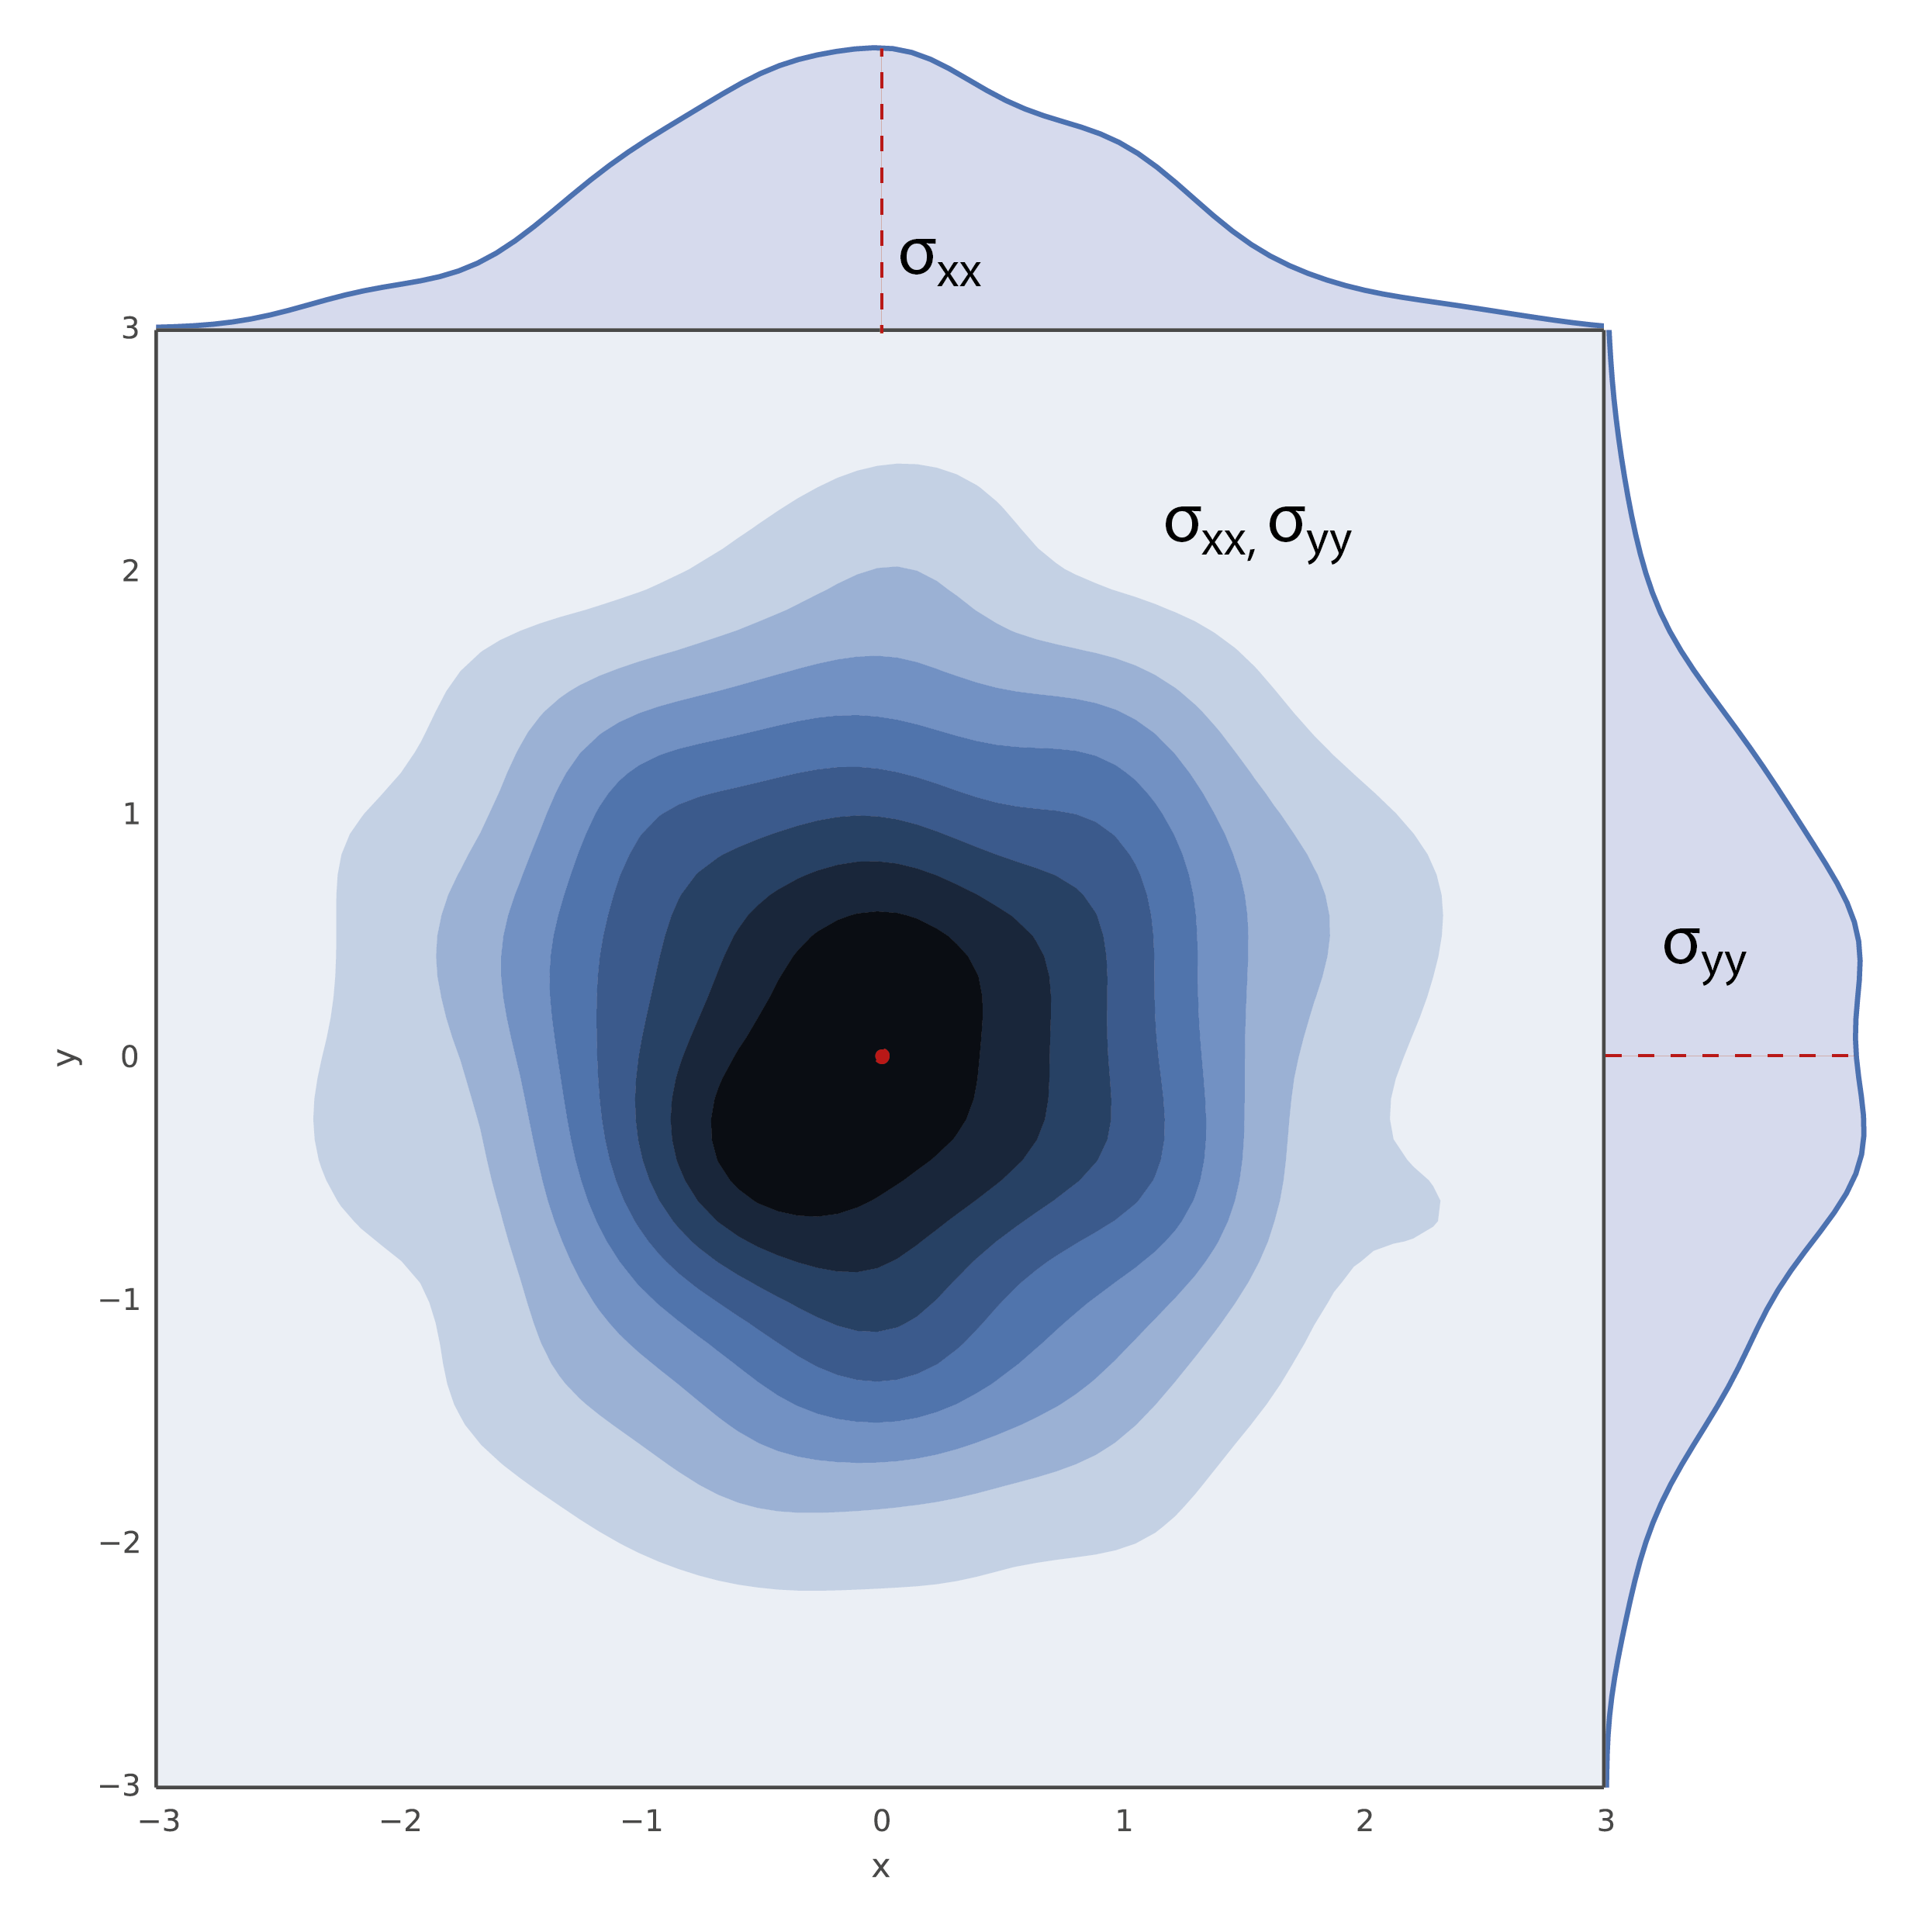
\includegraphics[scale=0.3]{chapterABCFlow/images/normal_sigma_example.png}
\caption{Comparing 1D and 2D distributions.}
\label{fig:normal_example}
\end{figure}



 \subsubsection{Normal distribution}
Here, we simulate two normal distributions, with $\mu=0$ and $\sigma=1$ 1000 times and measure the distance. In the 2D case, we simulate two multivariate normal distributions, with $\mu=0$ and covariance=[0.5 0, 0 0.5]. In the 1D case the median of the epsilon distribution was 0.00196 and the variance 0.0016. In the 2D case the median was 3.41e-14 and the variance 1.97e-07. 

\begin{figure}[H]
\centering
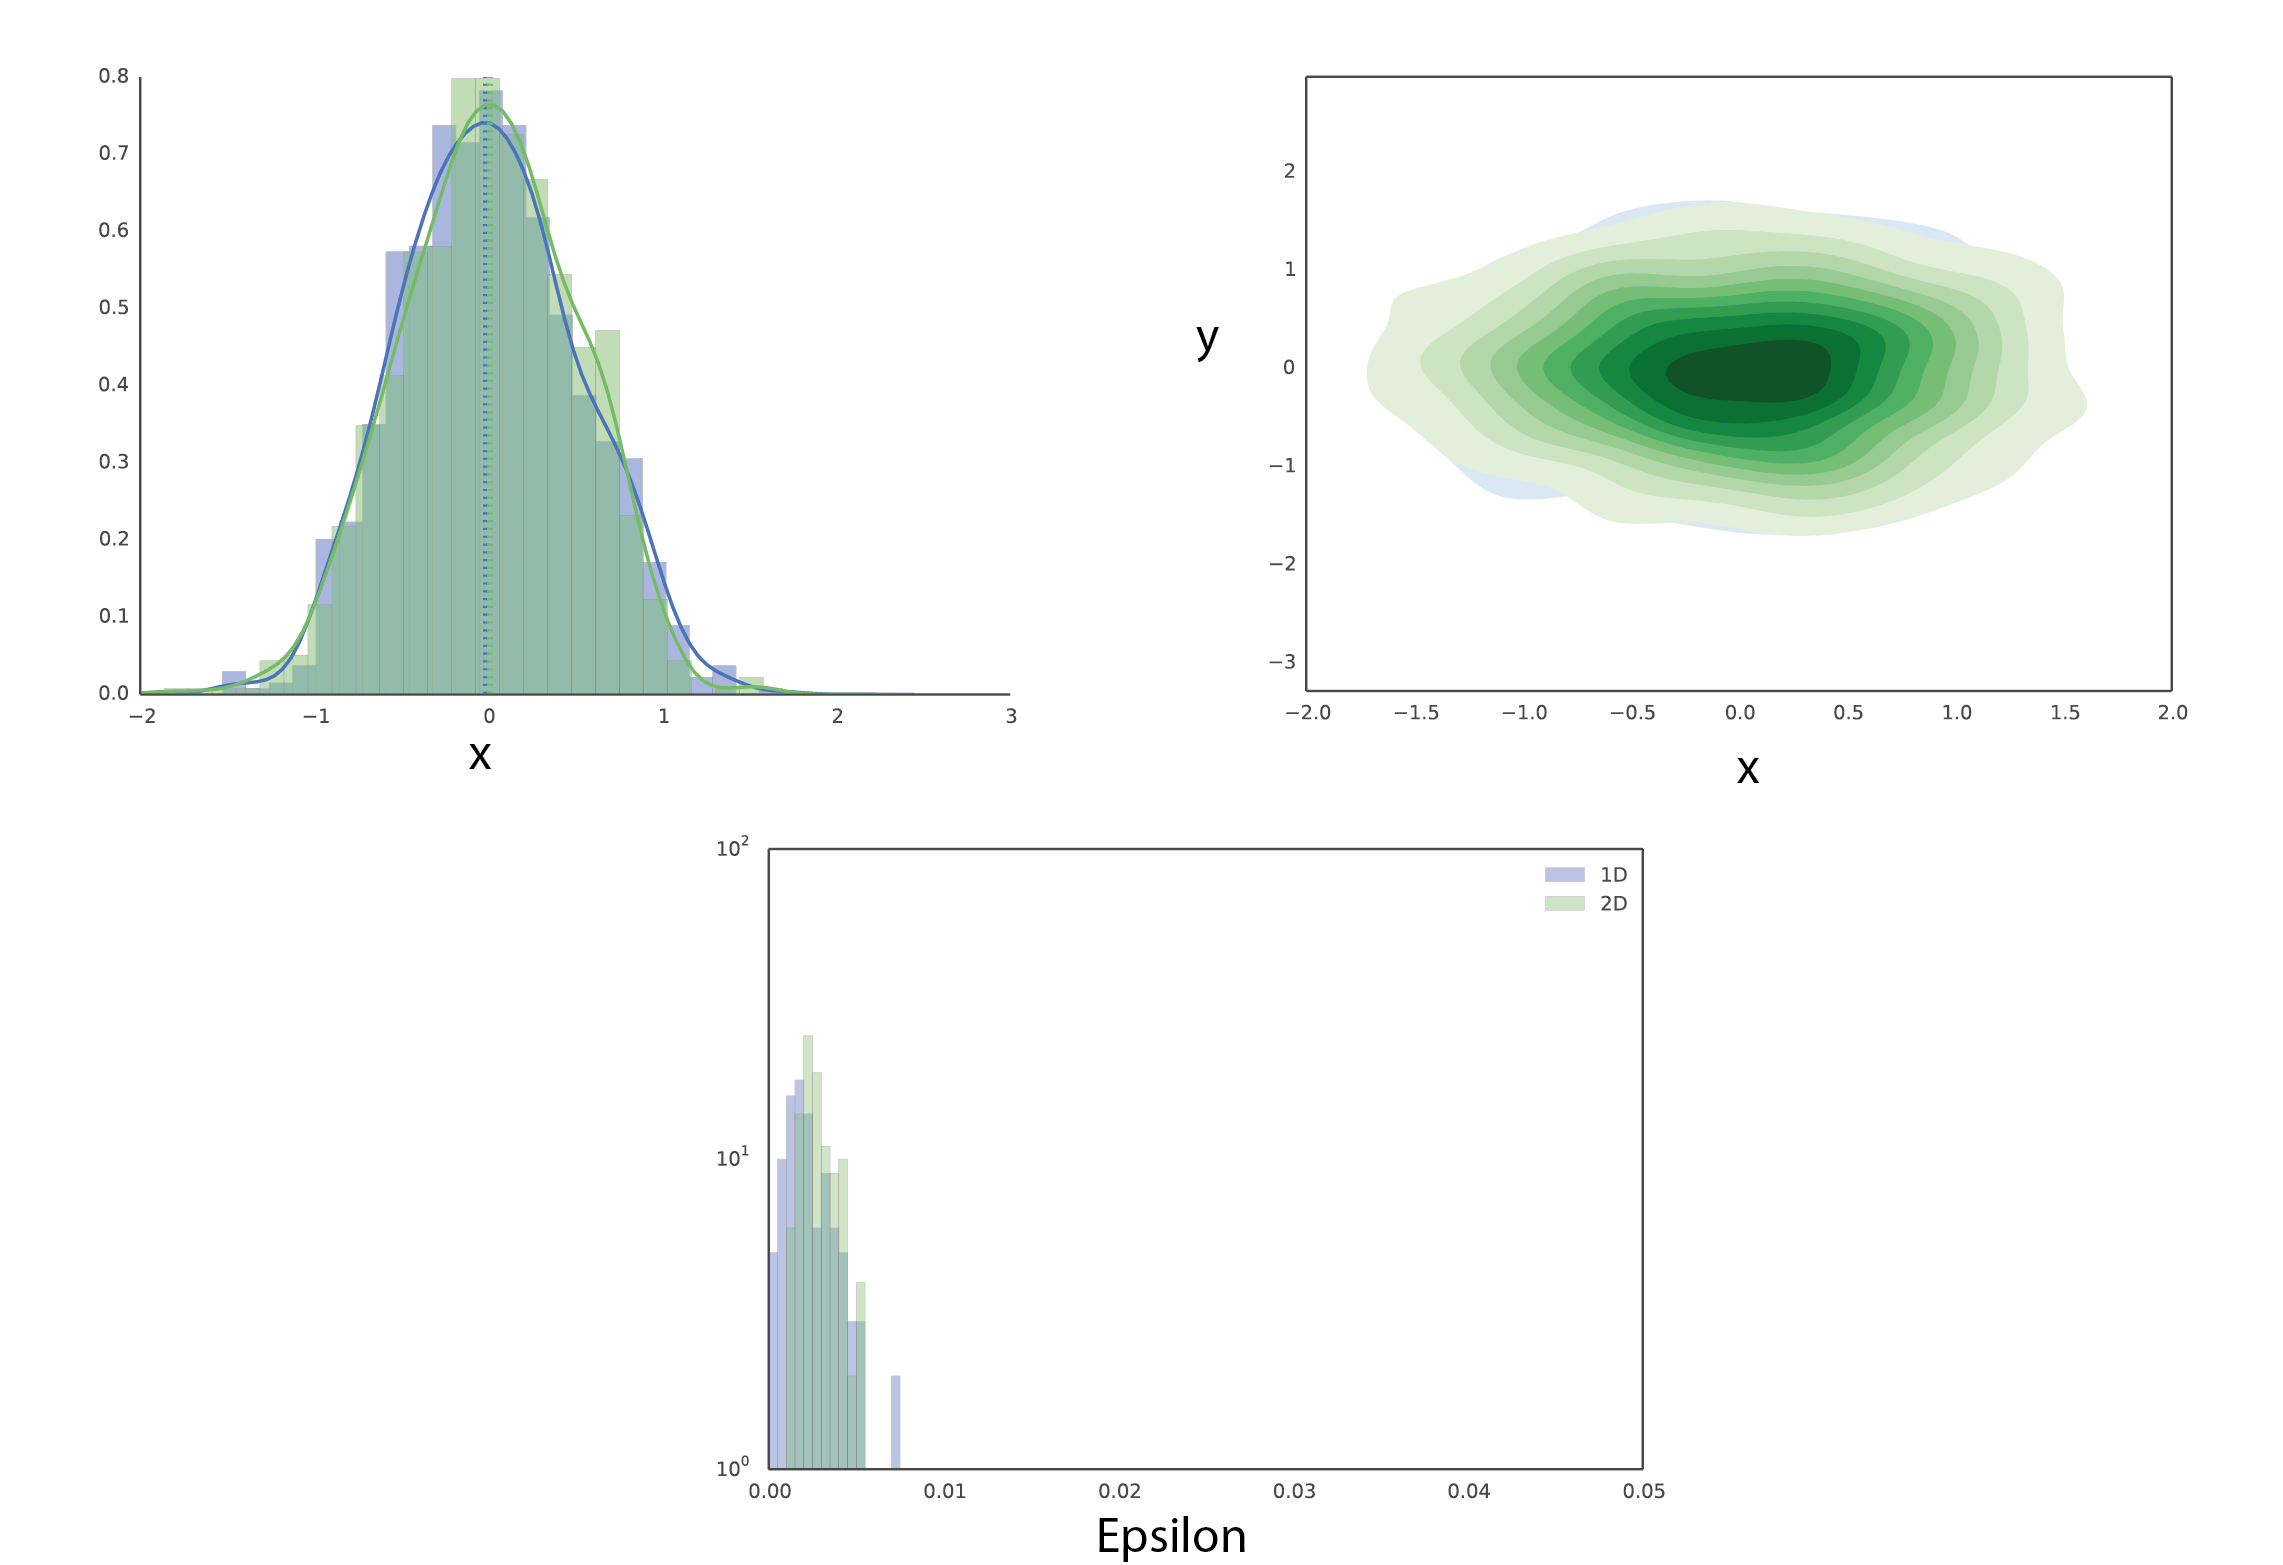
\includegraphics[scale=0.6]{chapterABCFlow/images/epsil_var.png}
\caption{Epsilon distribution for 1D (blue)  and 2D (green) distances.}
\label{fig:epsilon_hist}
\end{figure}

Next we study the effect that the number of data points have on the variance of the epsilons. 

\begin{figure}[htbp]
\centering
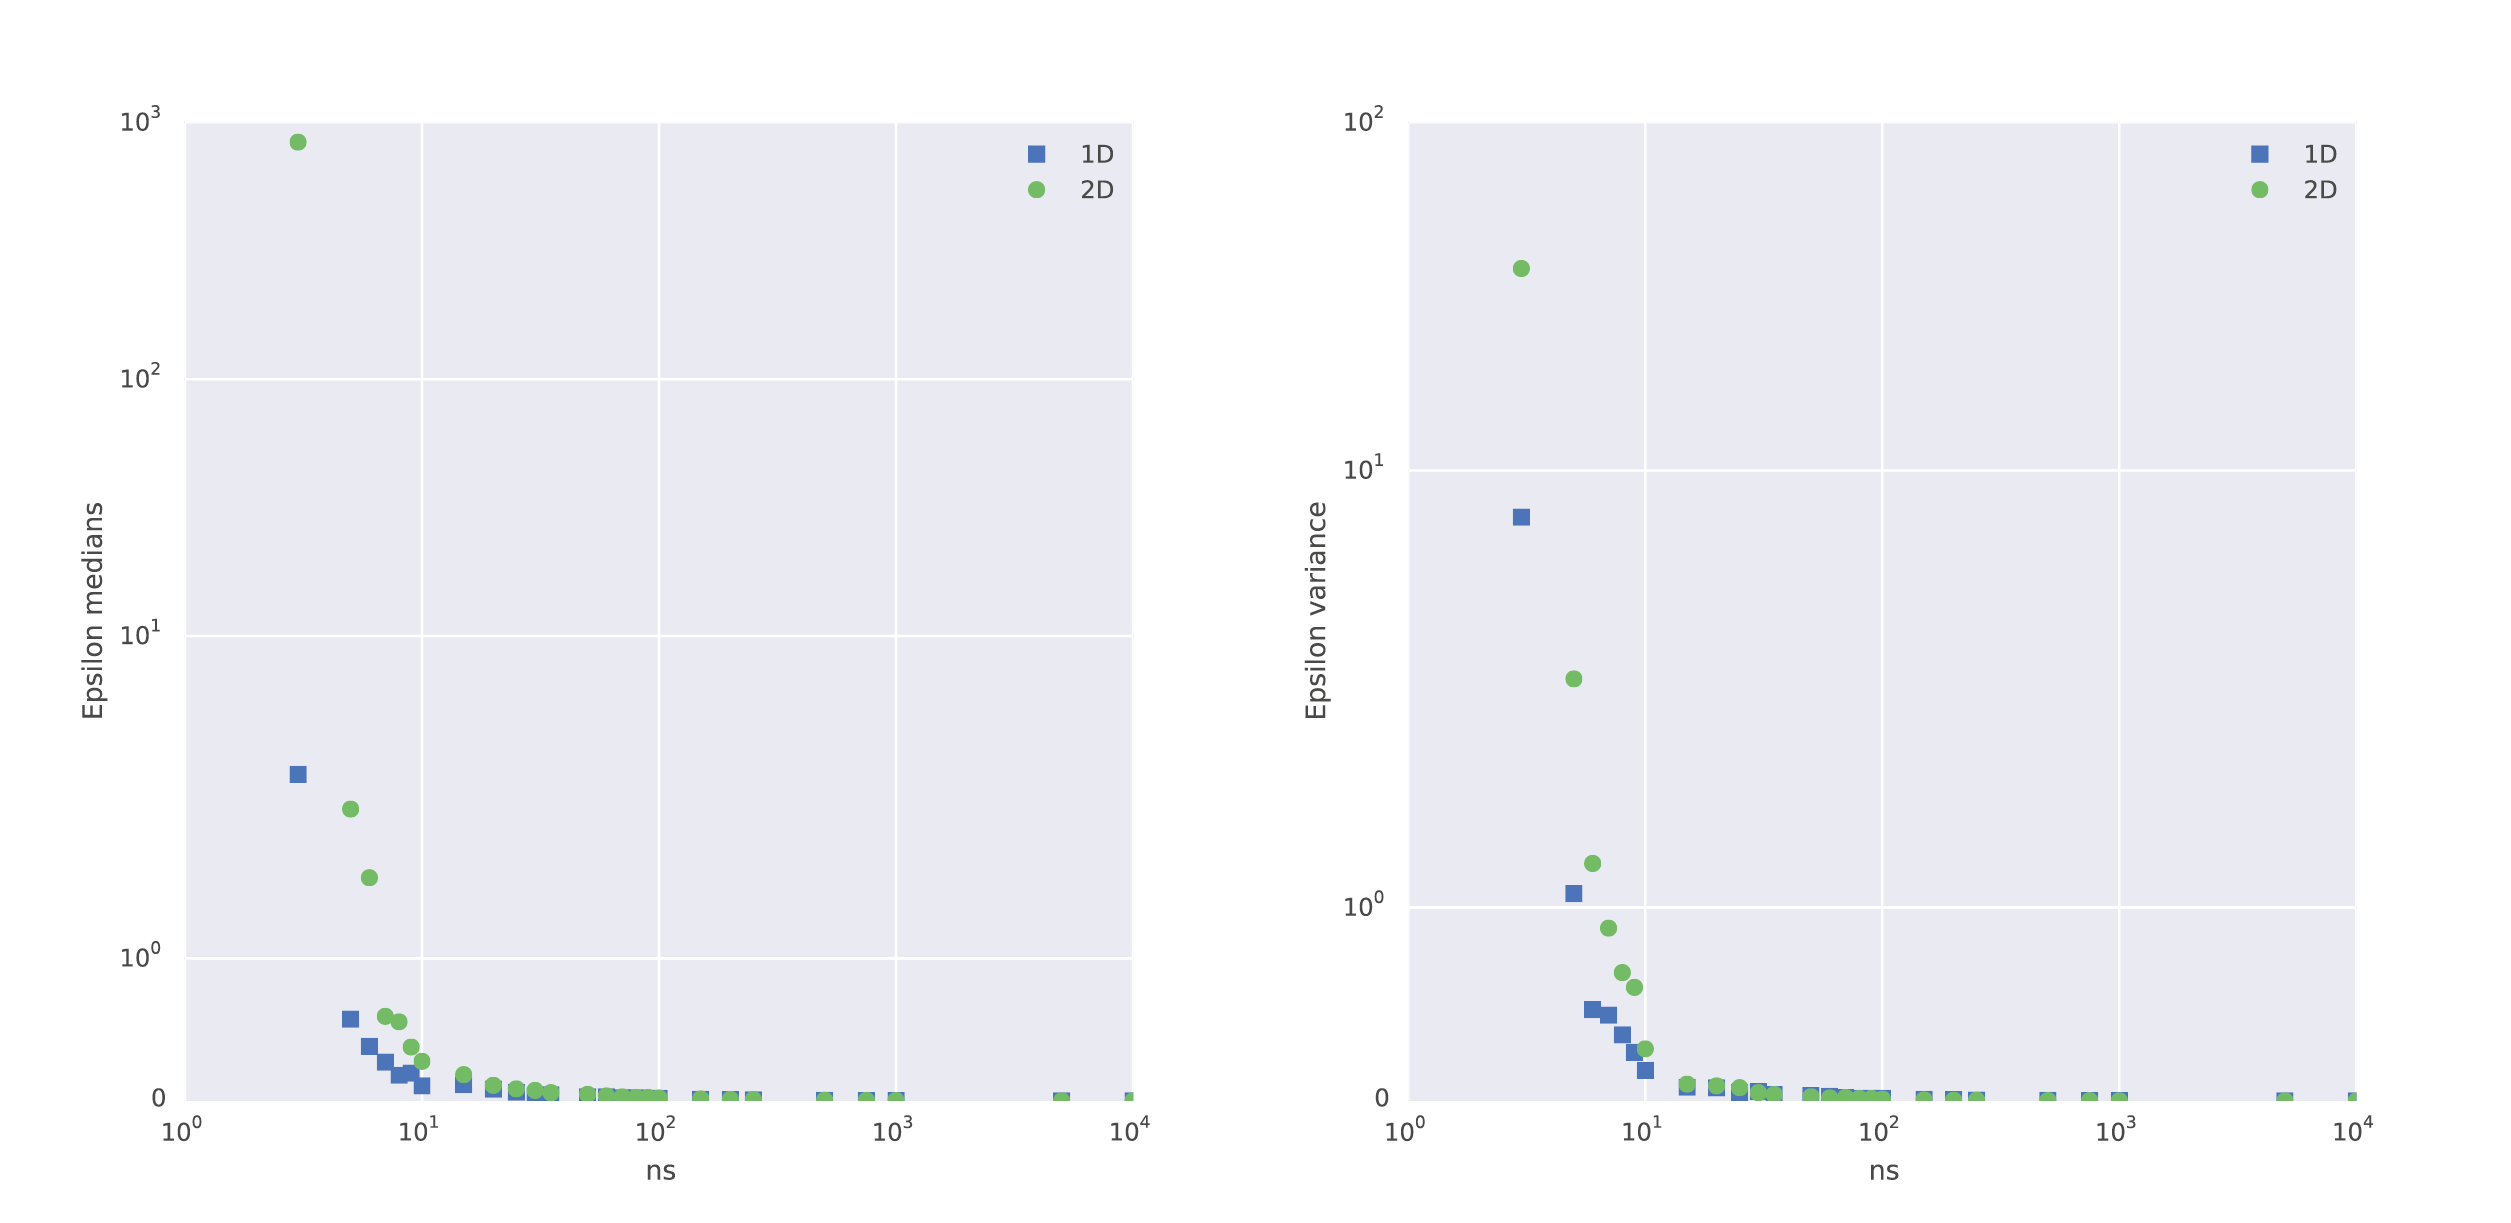
\includegraphics[scale=0.5]{chapterABCFlow/images/ns.png}
\caption{Epsilon distribution medians and variance over number of data points.}
\label{fig:epsilon_ns}
\end{figure}

As the number of data points increases, the distance calculation becomes more precise and more accurate. The median distance approaches zero, and the variance of the epsilon distribution decreases to zero. From Figure~\ref{fig:epsilon_ns} we conclude that the minimum number of data points  that need to be used to calculate the distance between the distributions in ABC-Flow is 100.  

The next parameter to be optimised is the bin size used in the distance calculation. In both 1D and 2D, the space is divided into bins, and the distance between corresponding bins in the data and the simulated data is calculated. The overall distance between to distributions is the sum of the distances between corresponding bins. %If the bin size is too large, small differences between 


\begin{figure}[htbp]
\centering
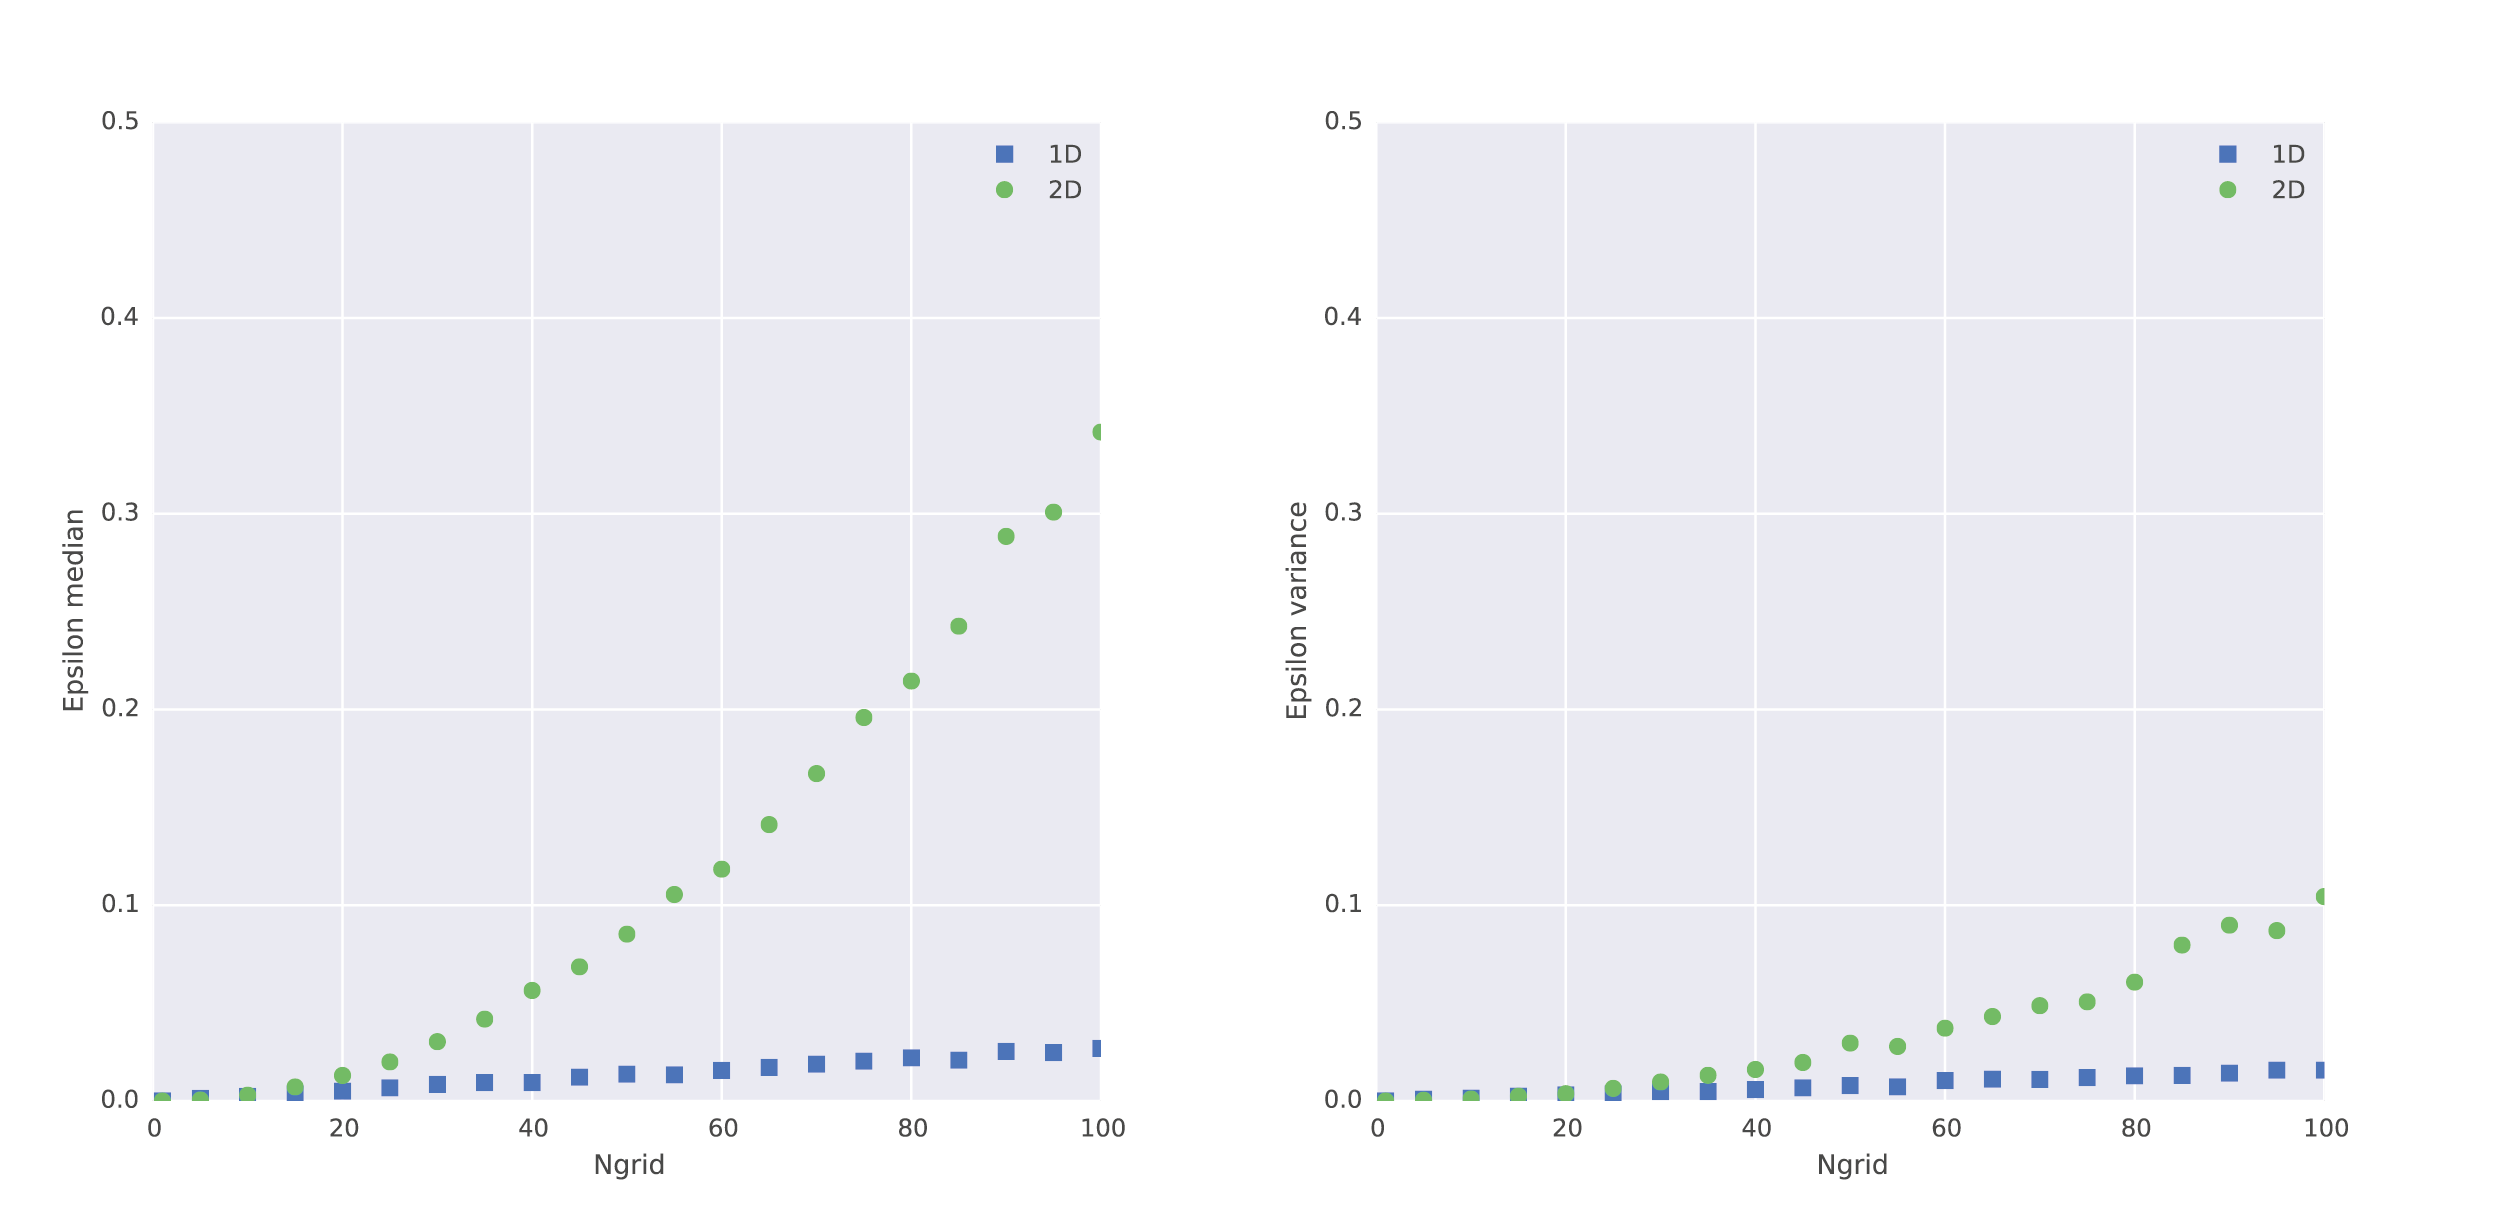
\includegraphics[scale=0.5]{chapterABCFlow/images/ngrid.png}
\caption{Epsilon distribution medians and variance vary with the size of bins used. }
\label{fig:epsilon_ngrid}
\end{figure}


We find that the 2D distance is more sensitive to the bin size than the 1D distance. From Figure~\ref{fig:epsilon_ngrid} we conclude that for a sample size of 100 data points, the optimal bin size for 1D and 2D distance calculation is 10. The above optimizations have been made by using standard normal distributions, of $\mu=0$ and $\sigma=1$. Here we investigate whether the distance calculation depends on the $\mu$ and $sigma$ of the distributions. 

\begin{figure}[htbp]
\centering
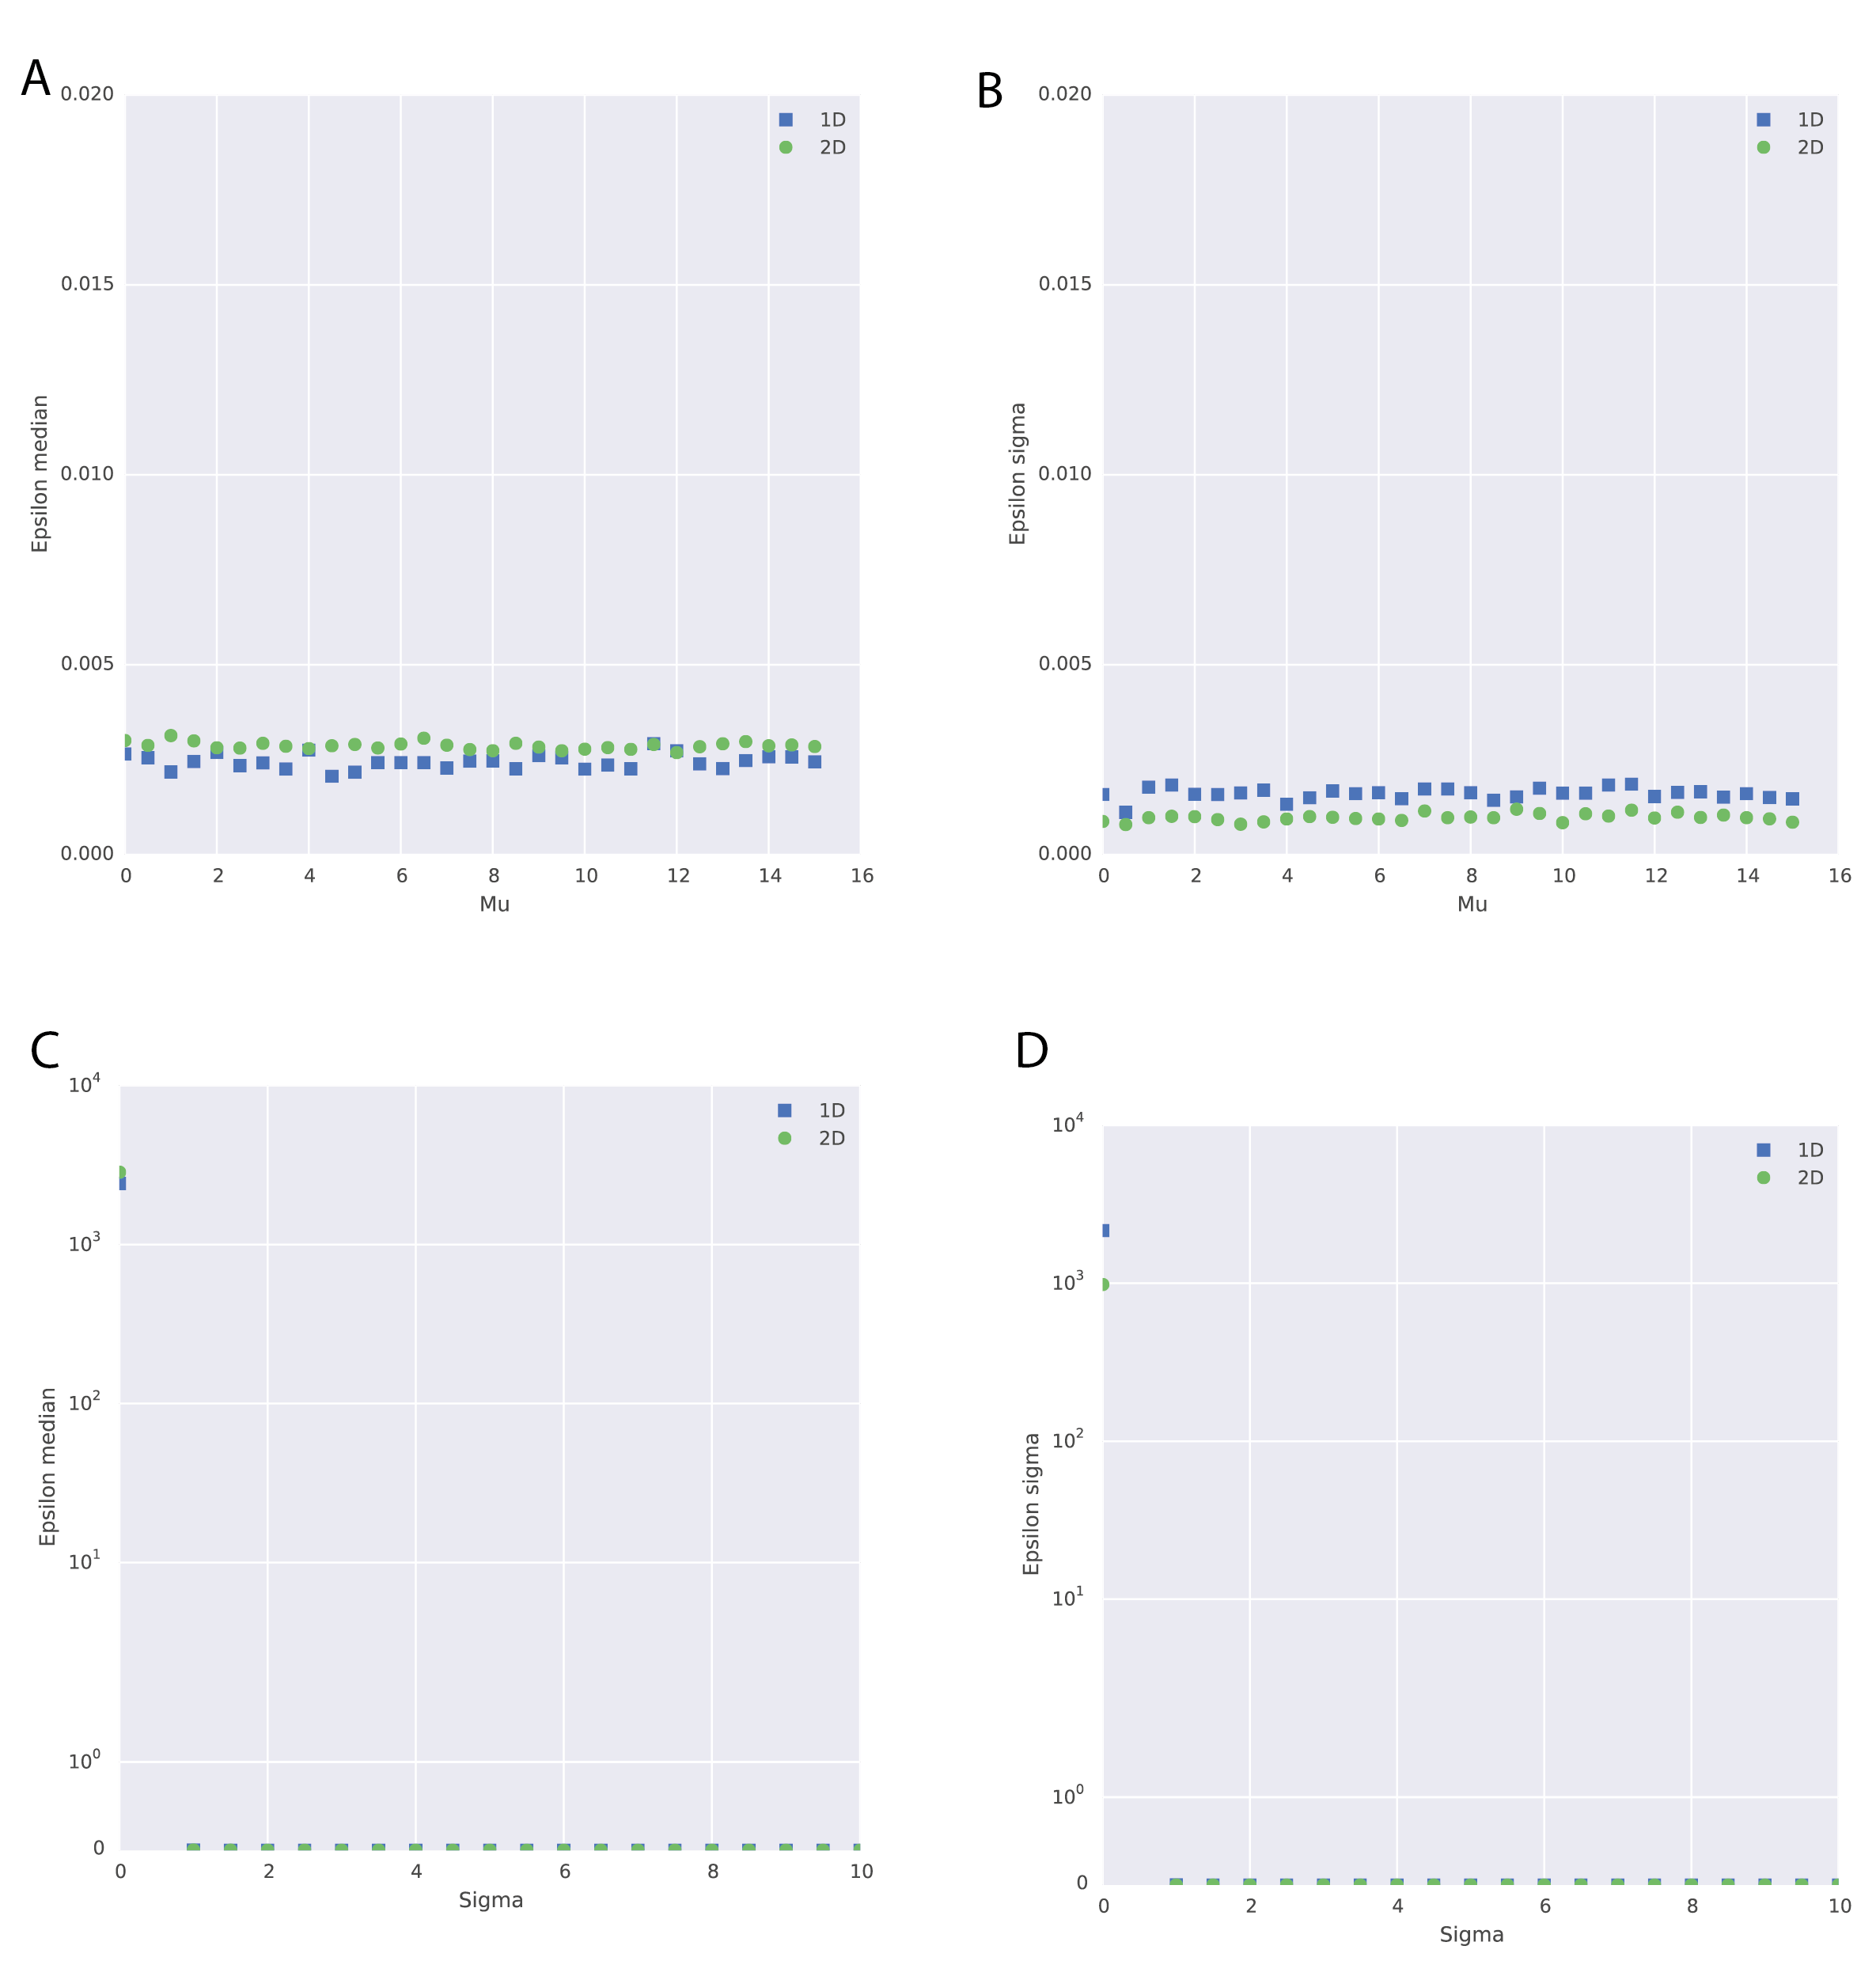
\includegraphics[scale=0.5]{chapterABCFlow/images/mus_sigmas_same.png}
\caption[LoF caption]{The distance calculations do not depend on the $\mu$ and $\sigma$ of the distributions. The median (A) and variance (B) of the epsilons remains constant with increasing $\mu$ (C,D) as well as with increasing $\sigma$. }
\label{fig:epsilon_mu_s_same}
\end{figure}
\clearpage
Next, by varying the amount of $\mu$ and $\sigma$ by which the two normals differ, we can find out the dynamical range of the epsilons. Whether two distributions are identical or vary by a large amount, we can get an estimate of how much the epsilon will vary from one to the other, both in 1D and 2D. 

\begin{figure}[htbp]
\centering
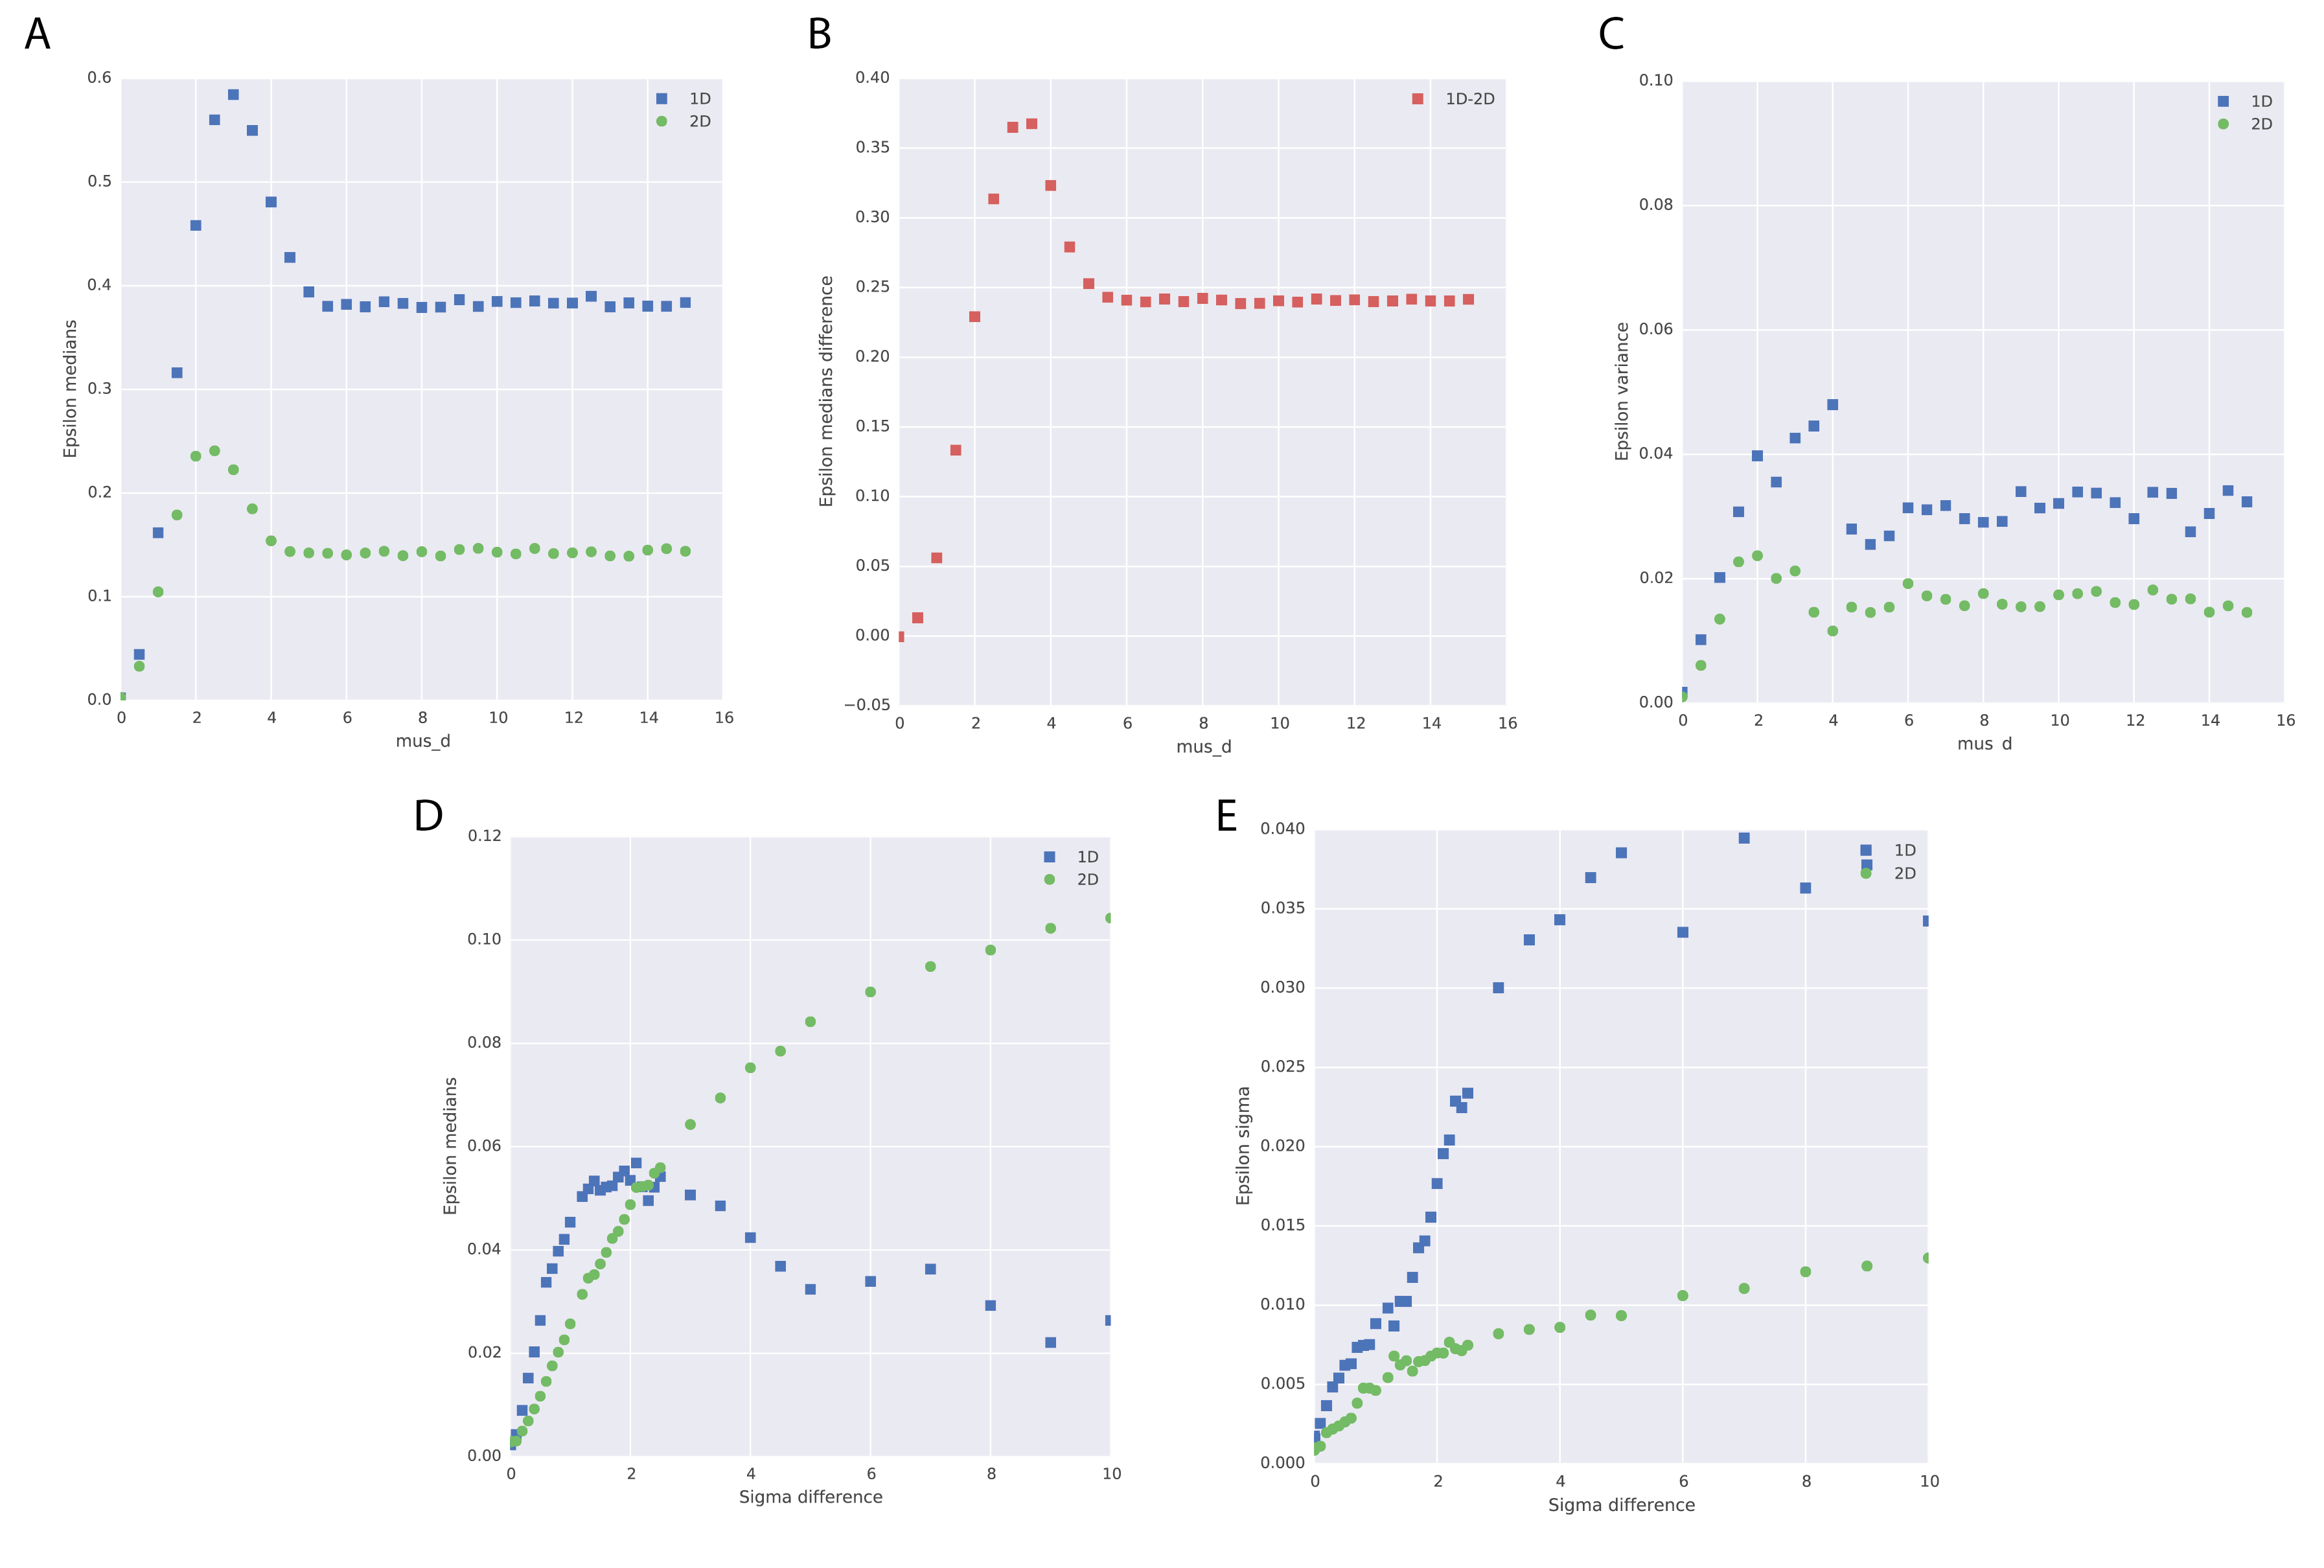
\includegraphics[scale=0.5]{chapterABCFlow/images/mus_sigmas_diff.png}
\caption[LoF caption]{ (A)The range by which epsilon varies as the difference between the $\mu$ of the distributions increases. (B) The difference between the epsilon distribution medians in the 1D and 2D case is not constant with increasing $\mu$ difference between the data sets. (C)The variance of the epsilon distributions remains relatively constant with increasing $\mu$. (D)The median of the epsilon distributions varies by a small amount with increasing difference in the $\sigma$ of the distributions, but the variance (E) remains relatively constant.}
\label{fig:epsilon_mu_s_diff}
\end{figure}
\clearpage



From Figure~\ref{fig:epsilon_mu_s_diff} we find that as the difference in $\mu$ increases the epsilon medians reach a plateau. We find that beyond a difference of 4 in $\mu$, the distance calculation cannot further separate the distances. This can be caused by the fact that when first dividing the space into bins, the range of the data is used to define the grid. If all the simulated data is located outside that grid, the algorithm can no longer distinguish between them, and will only allocate them as outside the range. The variance of the epsilon distributions does not vary significantly with increasing difference in $\mu$. As the difference in $\sigma$ increases between the distributions, we find that the median in the 2D distance calculation increases but not in the 1D. Note, that the range of the difference in the epsilon medians is small and thus we conclude that differences in the $\mu$ of a distribution are much better detected than the differences in the $\sigma$. The variance of the epsilon distribution when $\sigma$ is varied does not change significantly with increasing $\sigma$ difference.

\begin{figure}[htbp]
\centering
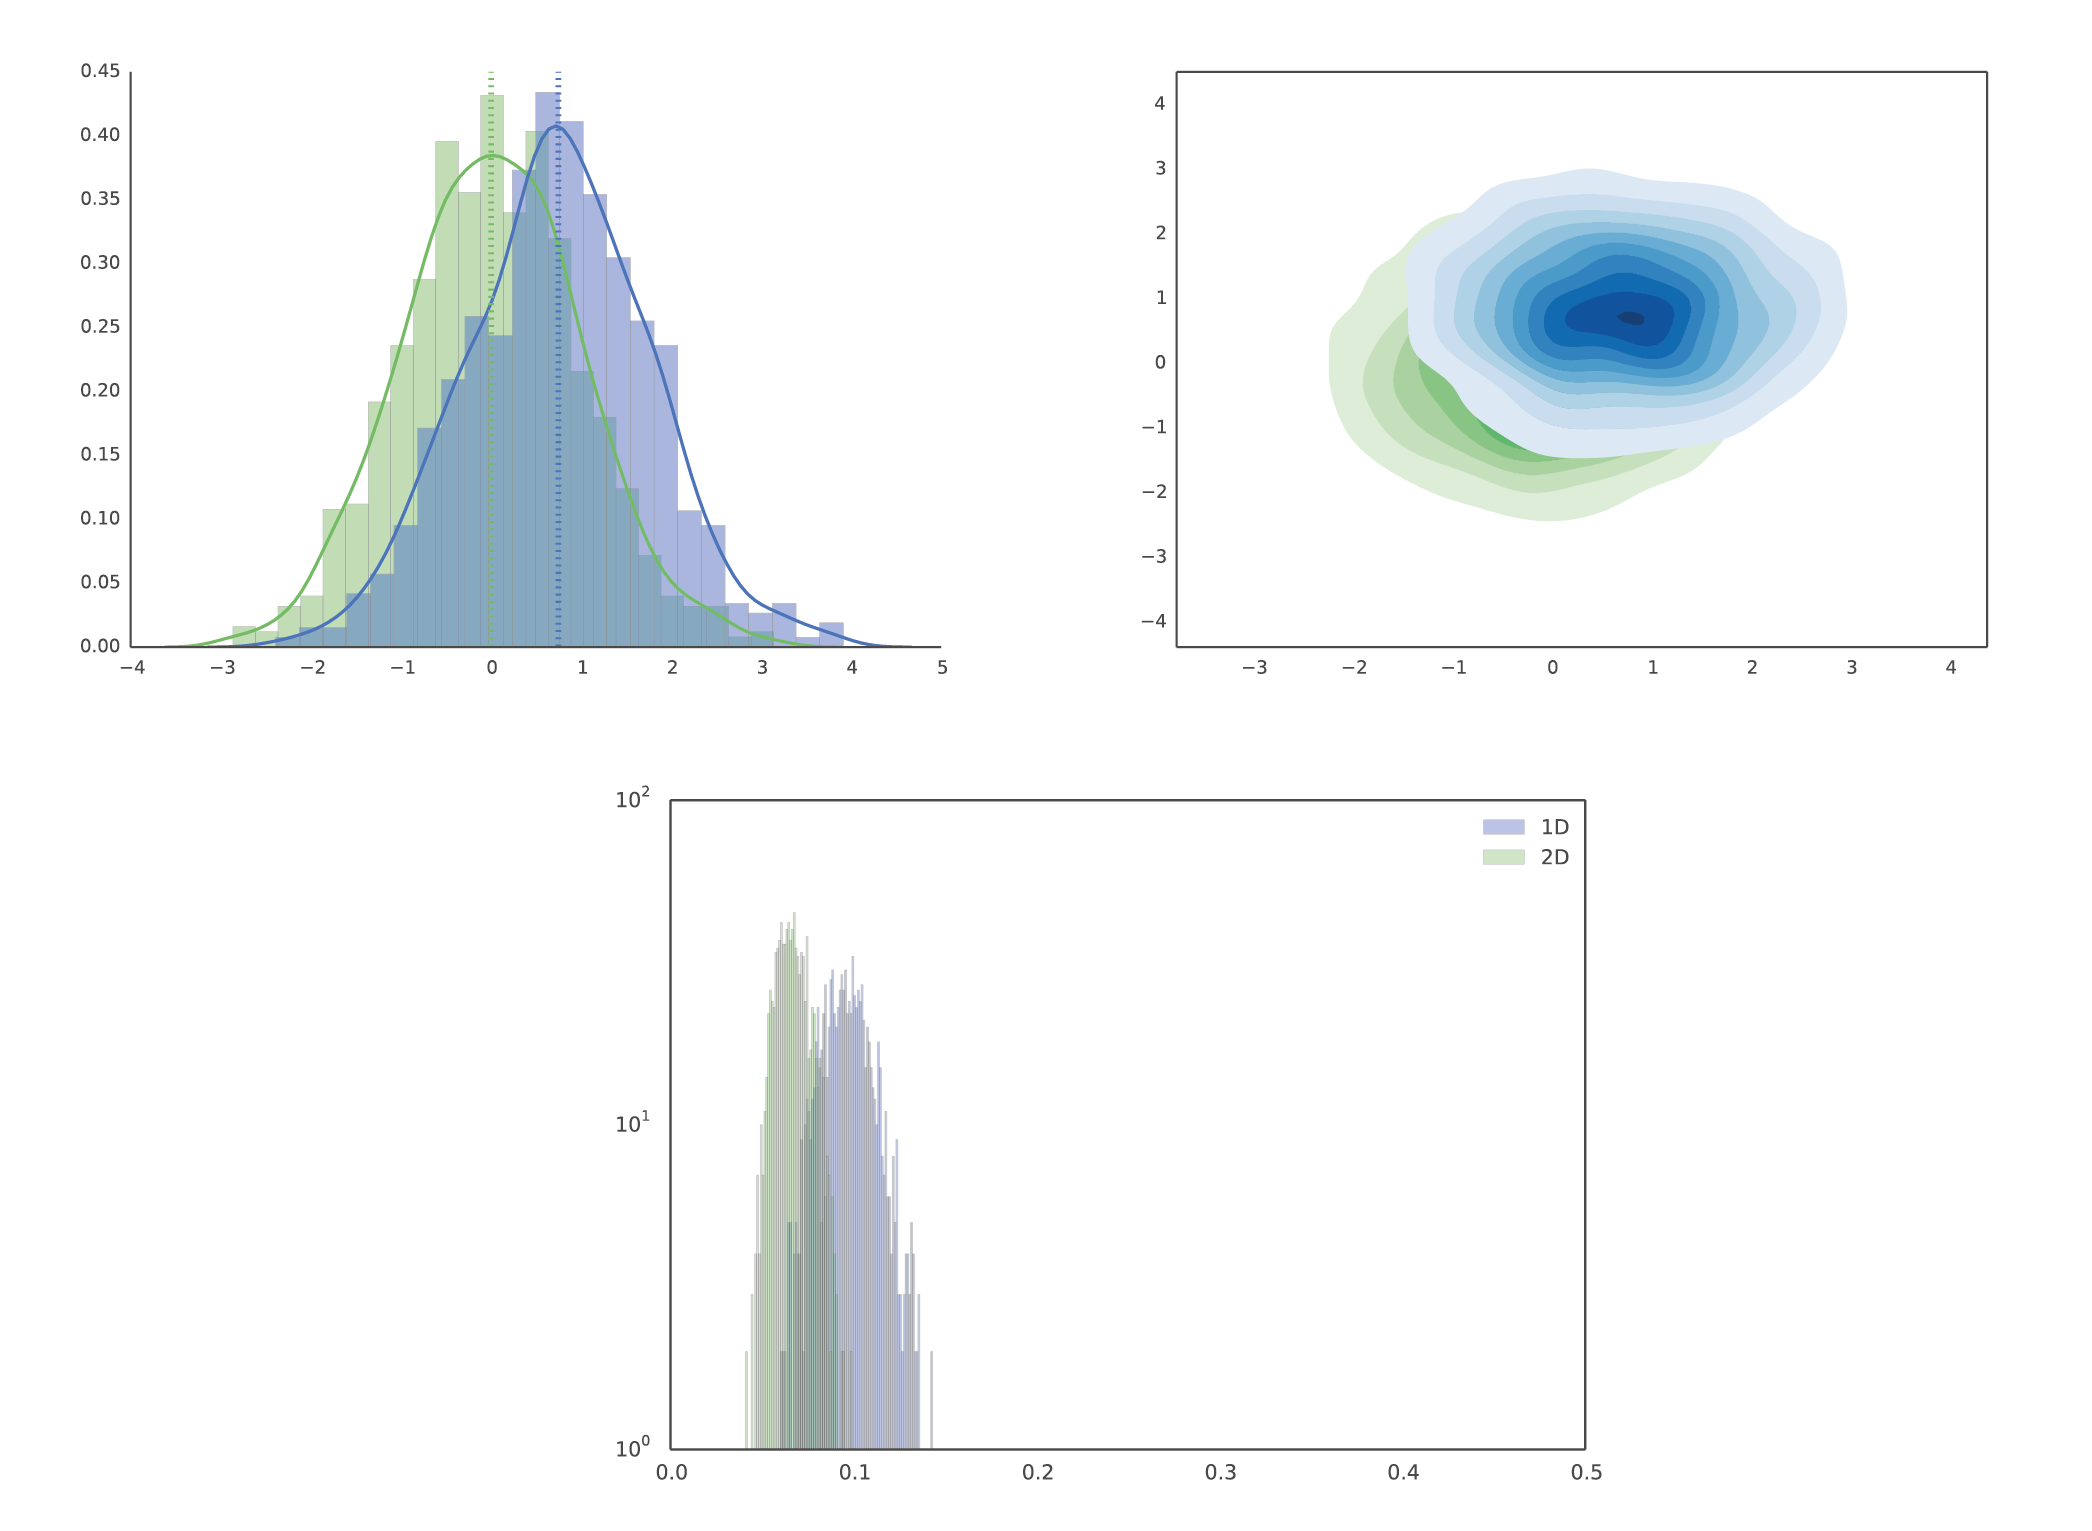
\includegraphics[scale=0.6]{chapterABCFlow/images/epsilon0-1.png}
\caption{The difference in distributions when epsilon median is smaller than 0.1 in 1D and 2D }
\label{fig:epsilon_0.1}
\end{figure}



\begin{figure}[htbp]
\centering
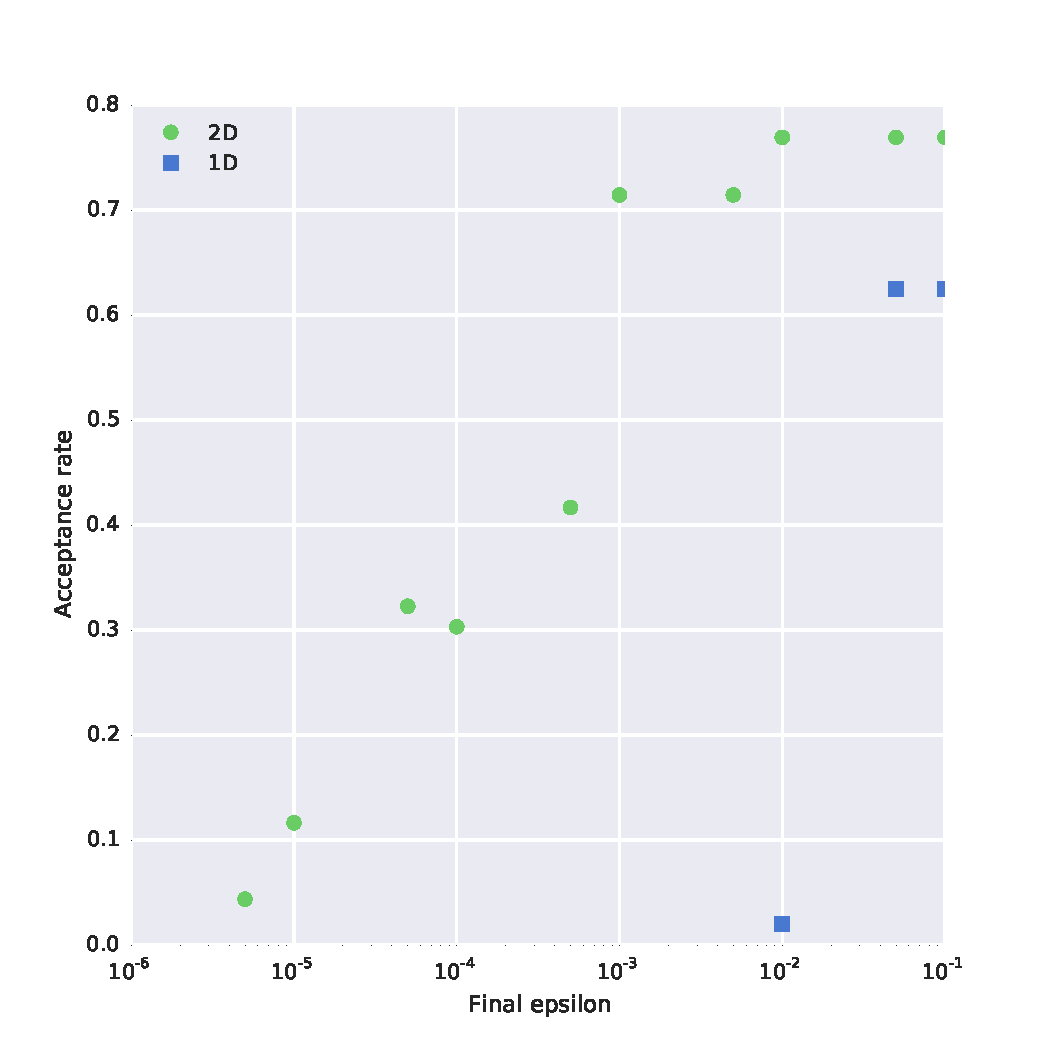
\includegraphics[scale=0.5]{chapterABCFlow/images/accept_rate_2d_1d.pdf}
\caption{Acceptance rate drops rapidly in the 1D case}
\label{fig:epsilon_acceptance_rate}
\end{figure}




\clearpage
 \subsubsection{Uniform distribution}

We study the epsilon distribution variance in the uniform distribution, [0, 1].  

\begin{figure}[htbp]
\centering
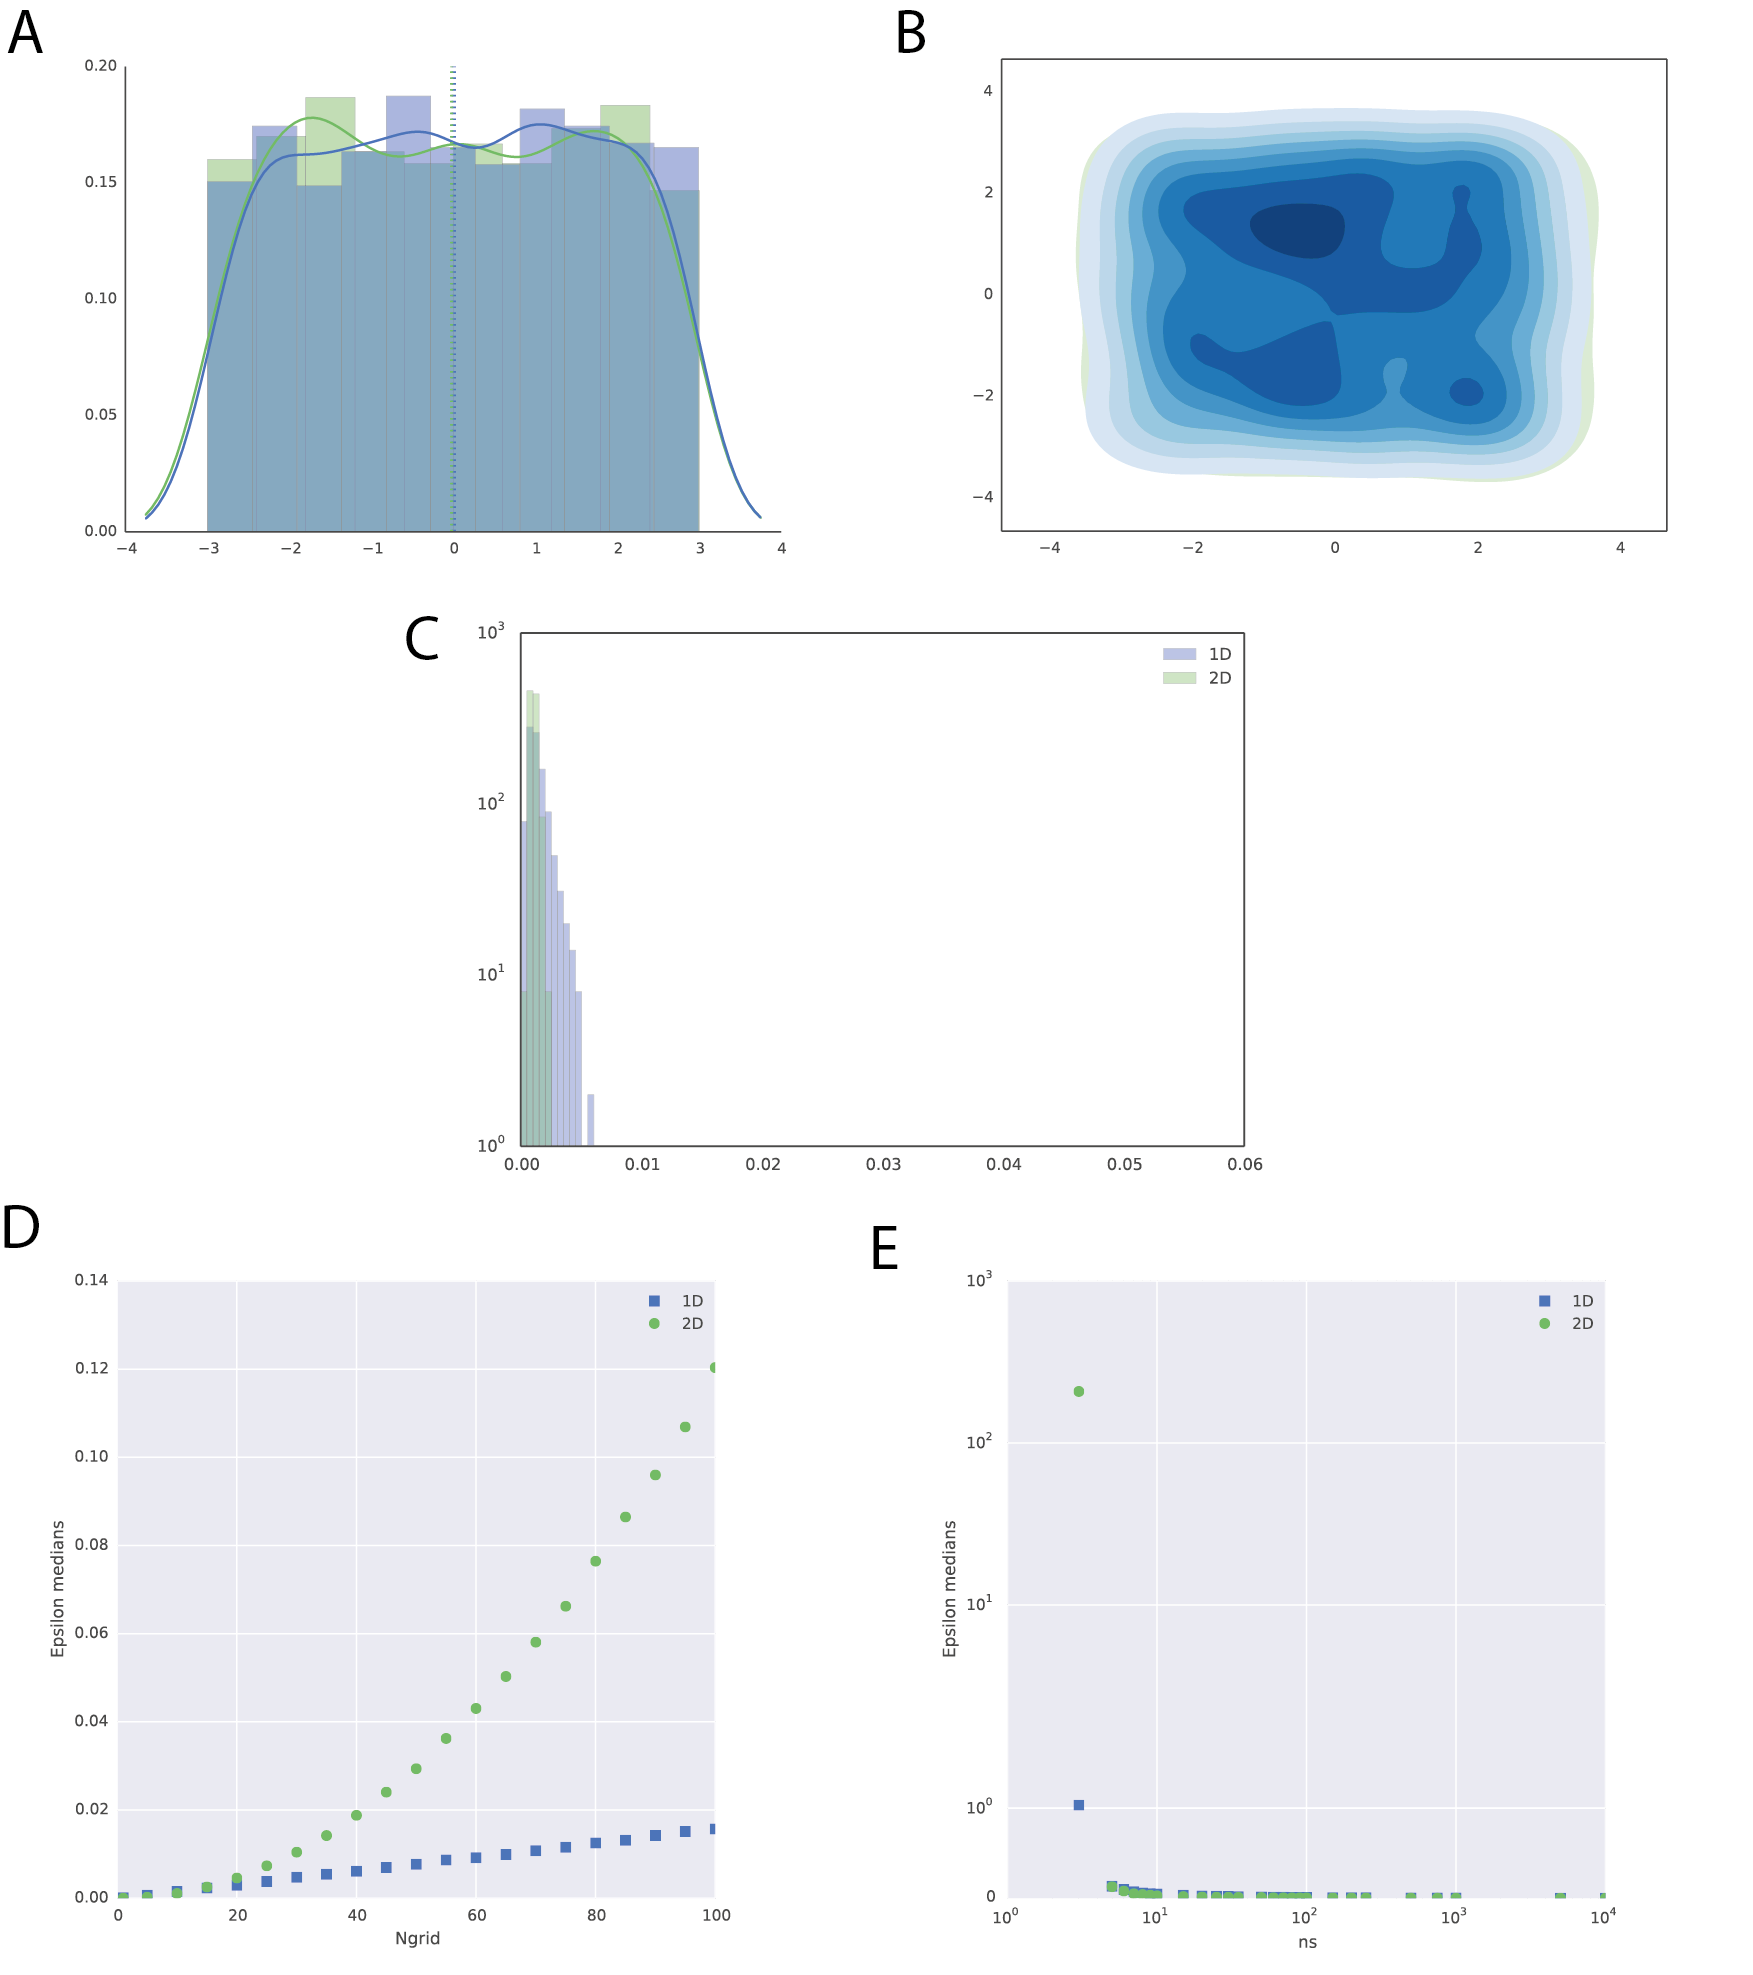
\includegraphics[scale=0.6]{chapterABCFlow/images/epsilon_uniform.png}
\caption[LoF caption]{Comparing the 1D and 2D distances between uniform distributions. (A) and (B) show samples of the uniform distributions compared in 1D and 2D respectively. (C) The epsilon distributions in the 1D and 2D distances are equivalent (D,E) Epsilon medians and variance varies with how dense the grid is in the 2D case.}
\label{fig:epsilon_uniform}
\end{figure}


 \subsubsection{Comparing uniform and normal distributions}
When comparing a normally distributed data set to a uniformly distributed data set, we don't see a great difference between the 1D and 2D epsilons.


\begin{figure}[htbp]
\centering
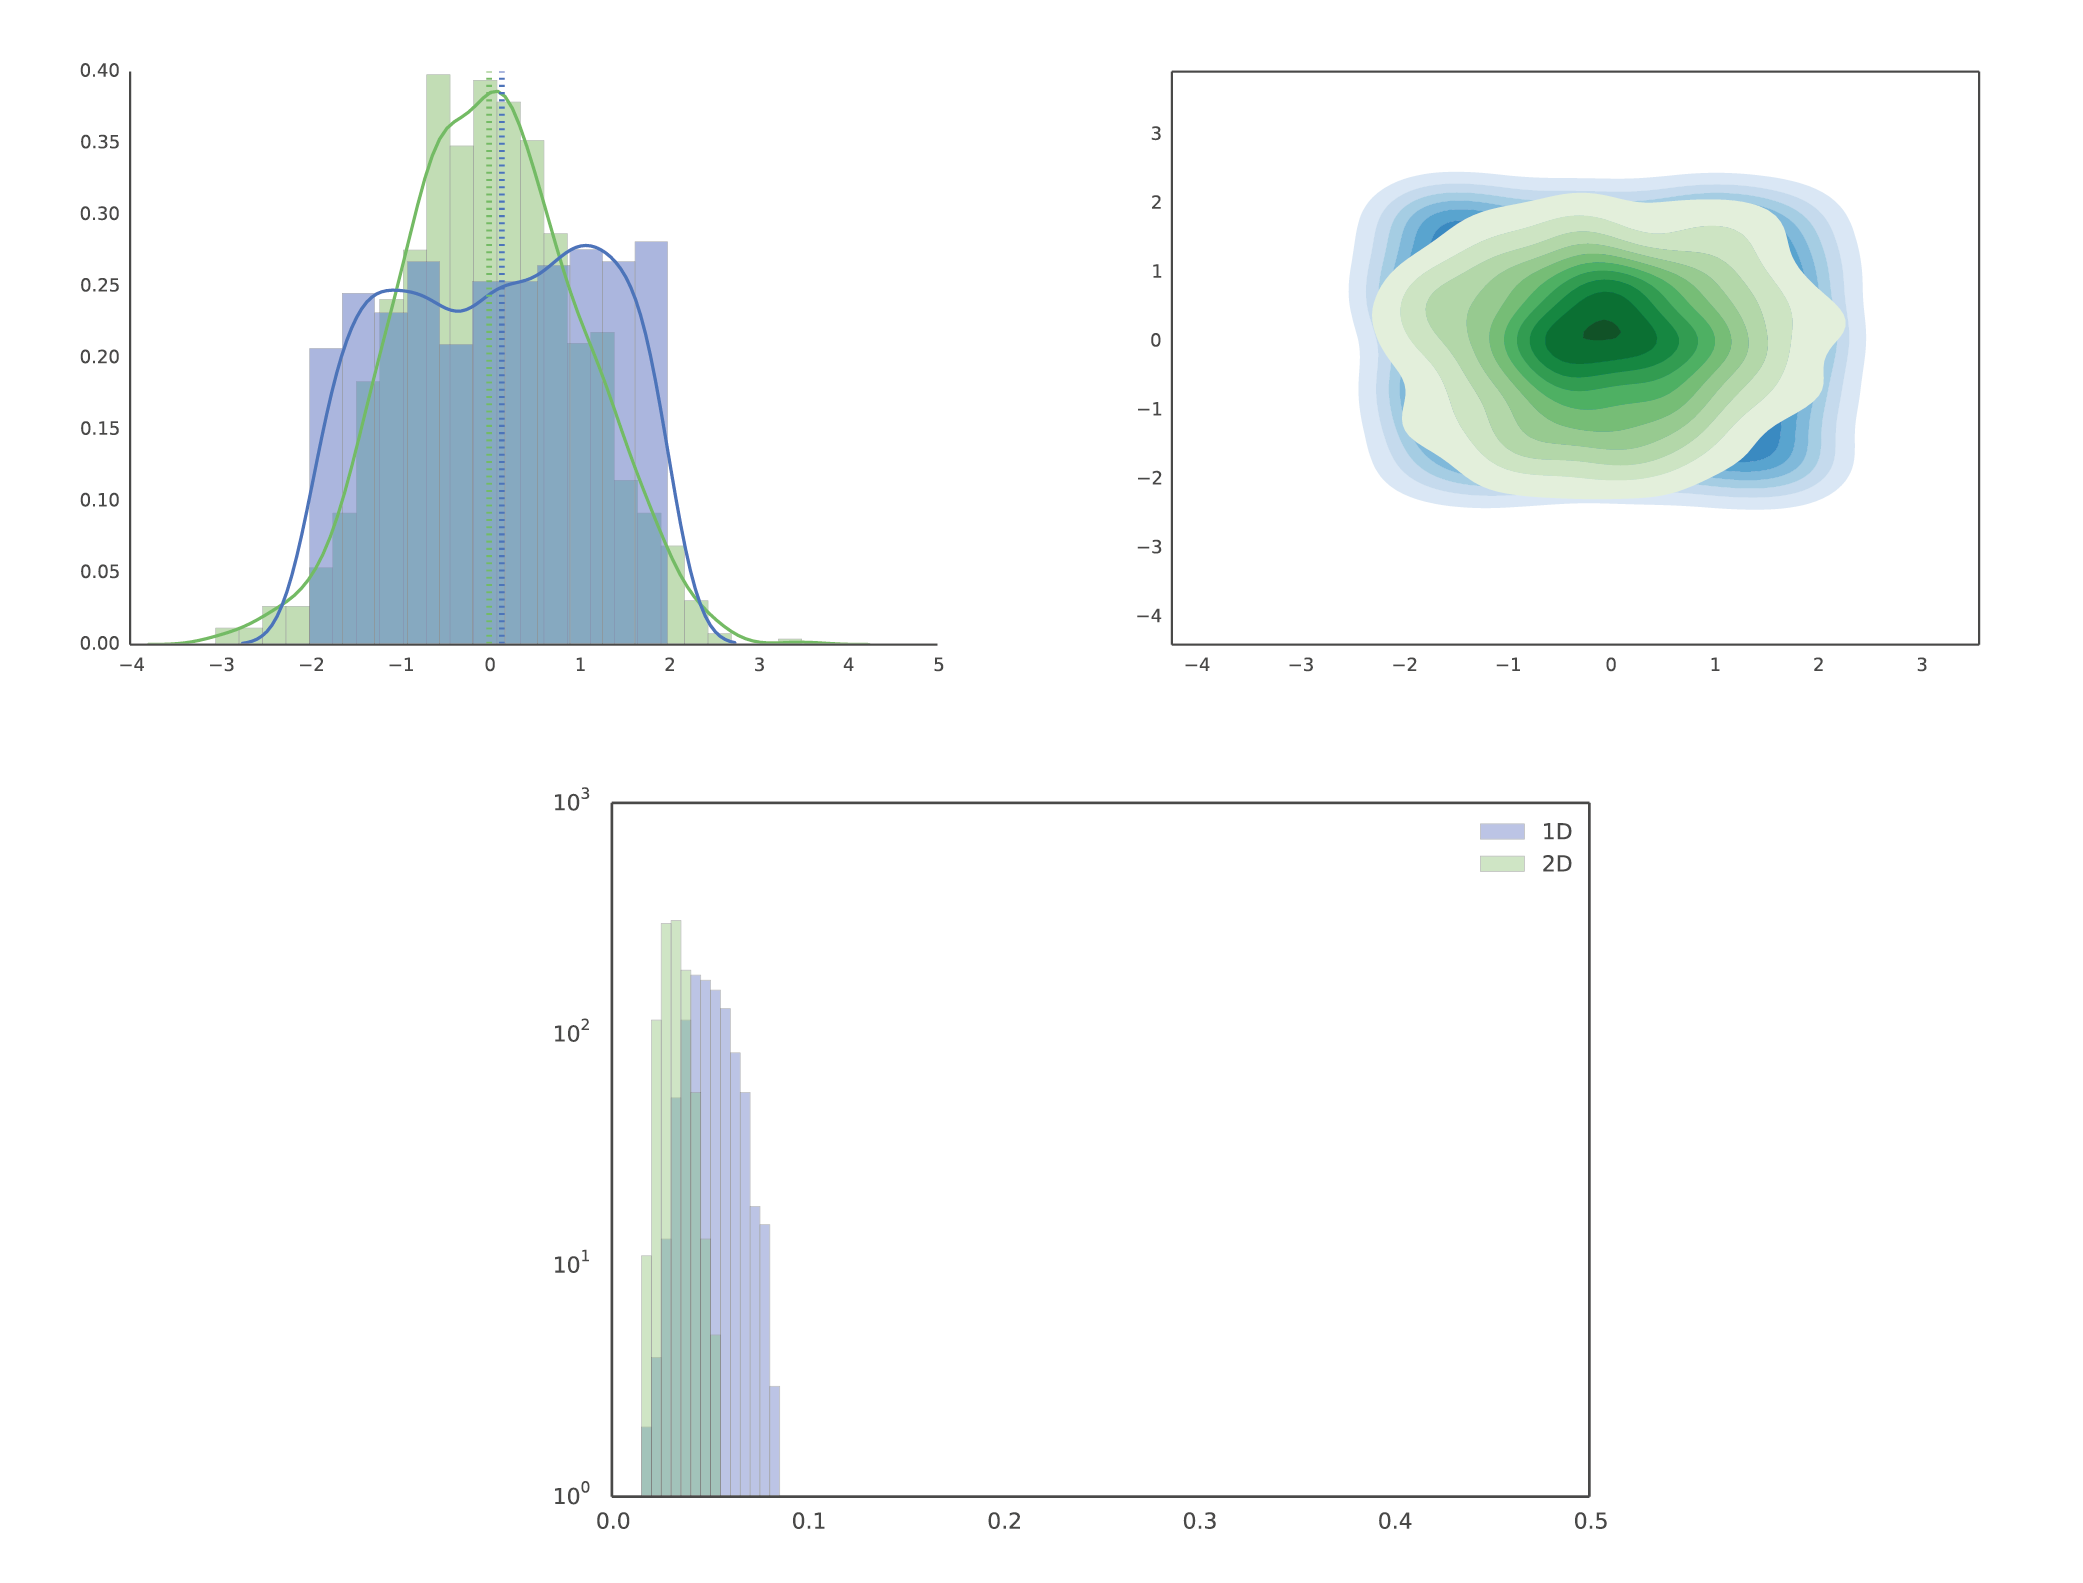
\includegraphics[scale=0.6]{chapterABCFlow/images/uni_v_normal.png}
\caption{Comparing normally distributed data to uniformly distributed simulations.}
\label{fig:epsilon_uni_v_normal}
\end{figure}
\clearpage


 \subsubsection{Bimodal distributions}
Another type of distribution that is commonly found in Flow cytometry experiments, is a bimodal distribution. Here we test whether the 1D and 2D distances are equivalent when measuring distances in this type of distributions.

\begin{figure}[htbp]
\centering
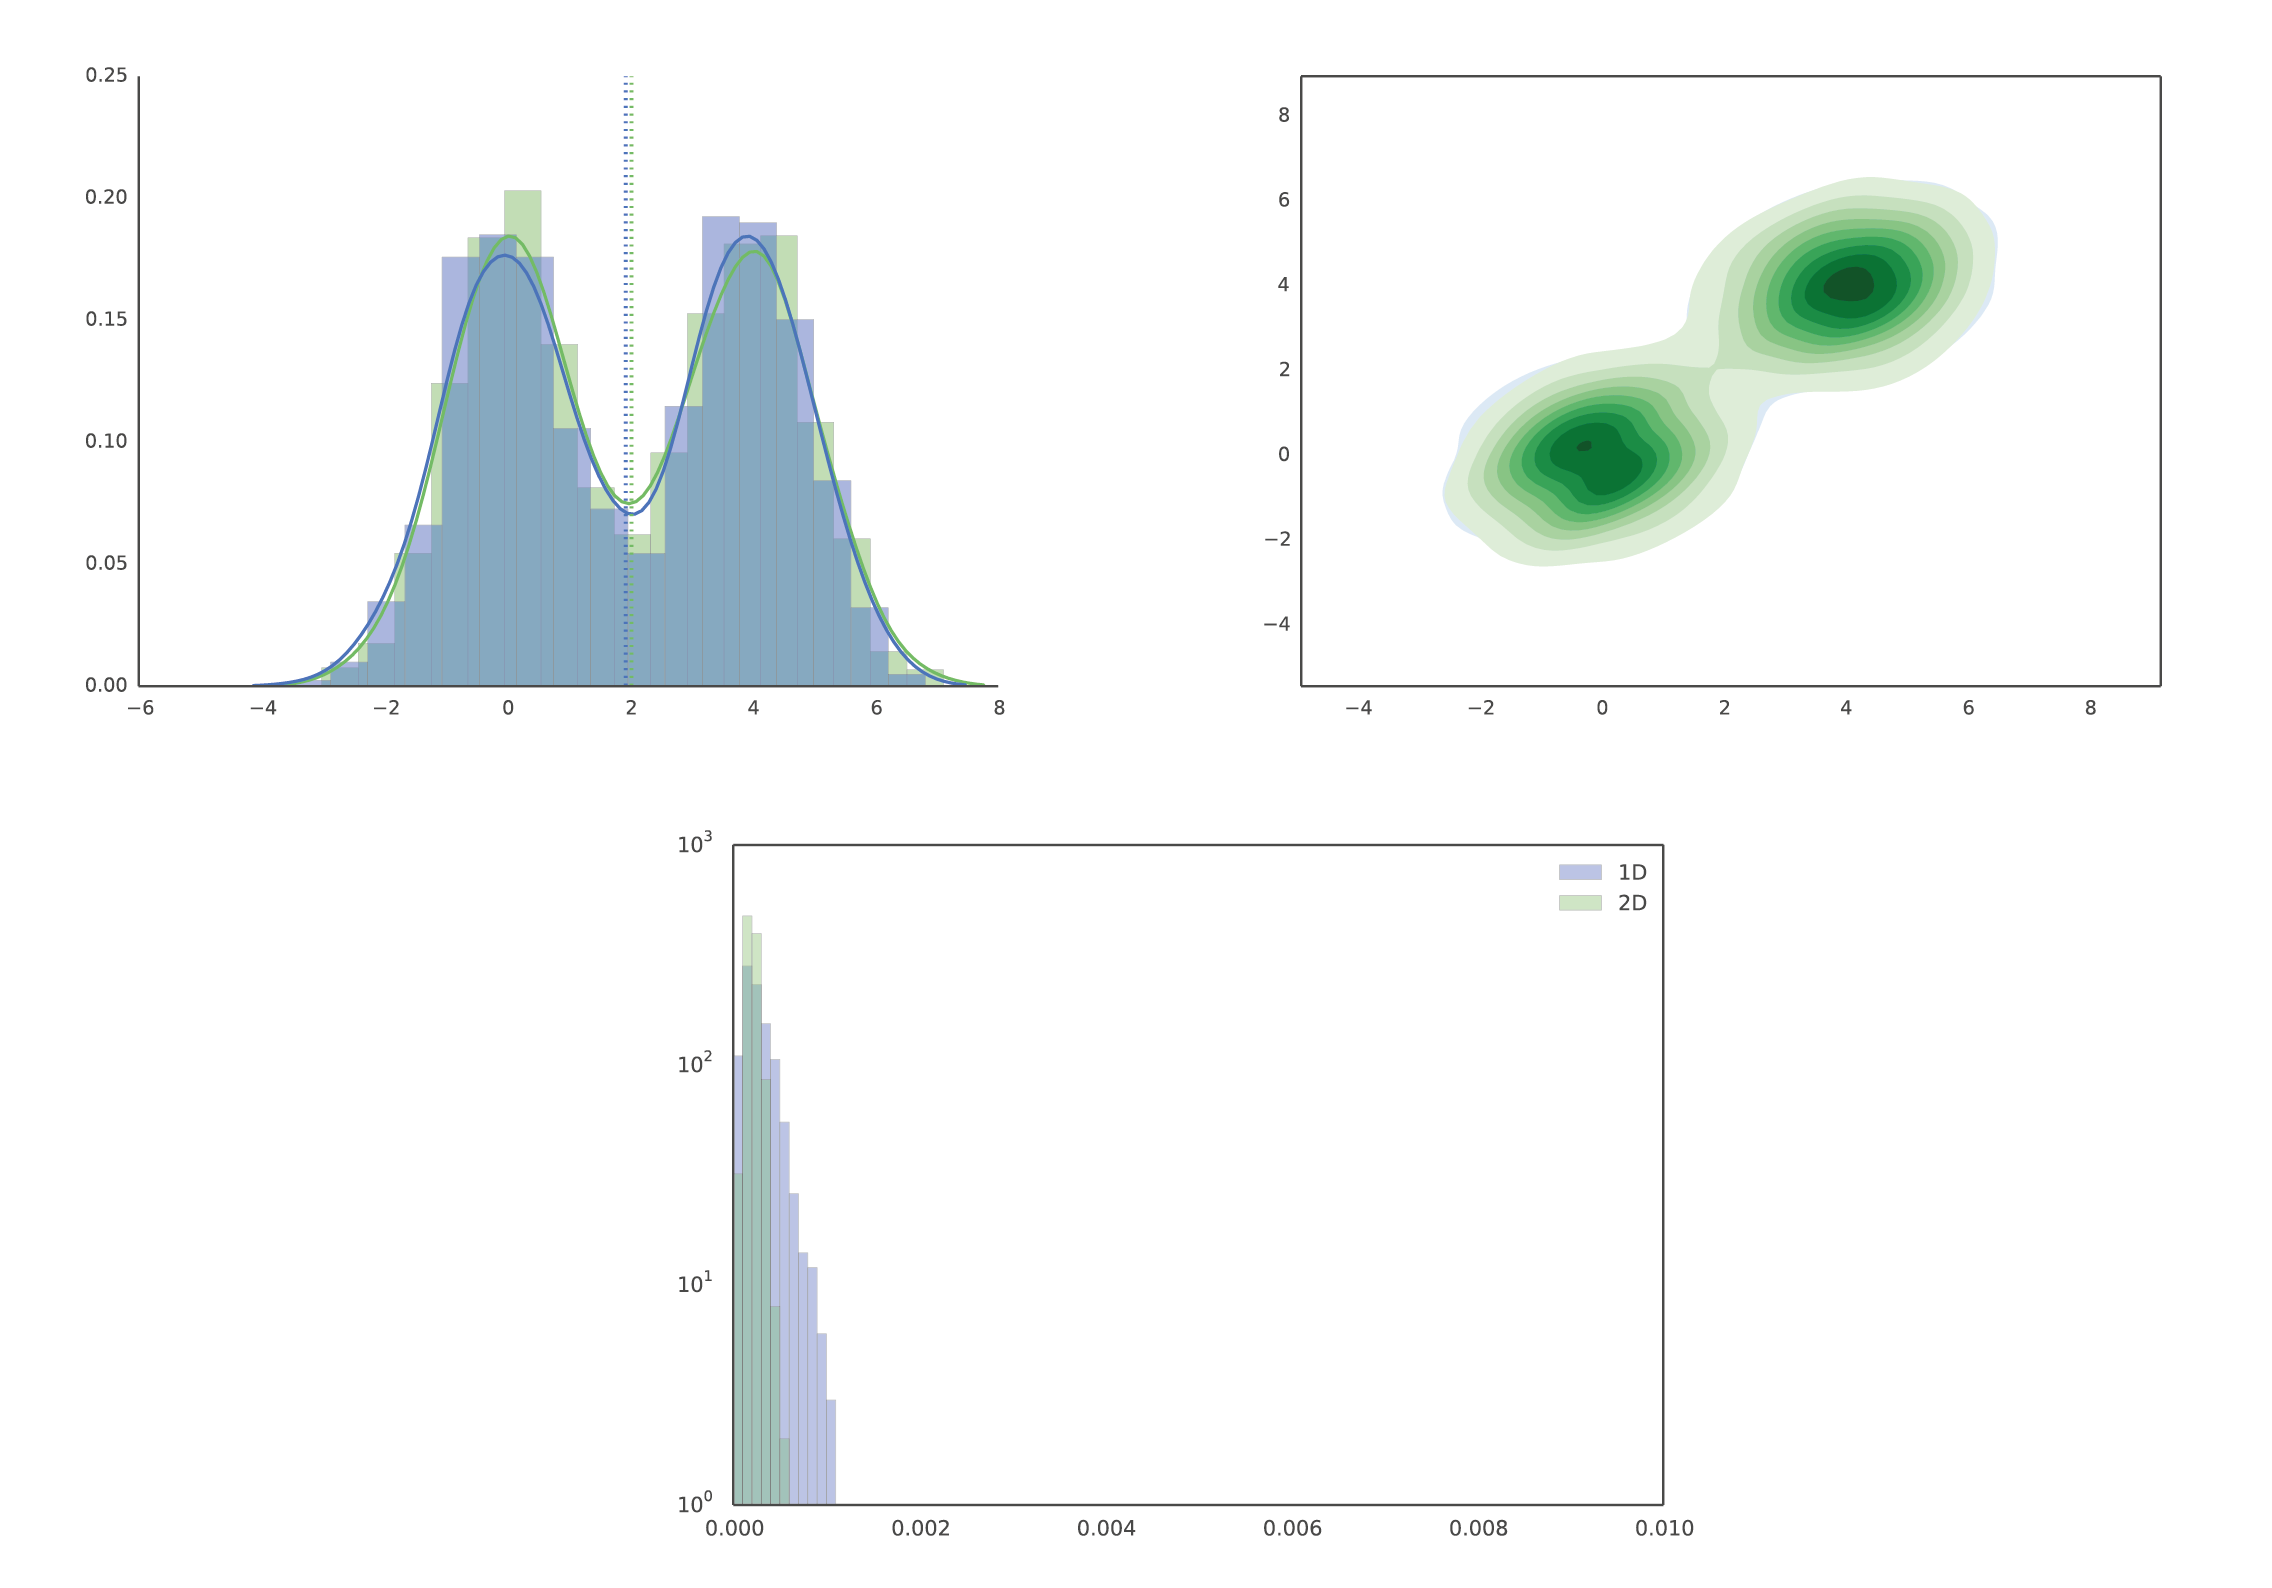
\includegraphics[scale=0.6]{chapterABCFlow/images/multimodal.png}
\caption{Comparing the 1D and 2D distances between bimodal distributions. }
\label{fig:multimodal}
\end{figure}
 We find that the two distances are comparable when dealing with this kind of distibution. Next, we examine how the distance between bimodal distributions with different $\mu$ varies in the 1D and 2D cases. We find a similar behaviour like the one observed when comparing normal distributions with increasinglt different $\mu$ (Figure~\ref{fig:epsilon_mu_s_diff}). 
\begin{figure}[htbp]
\centering
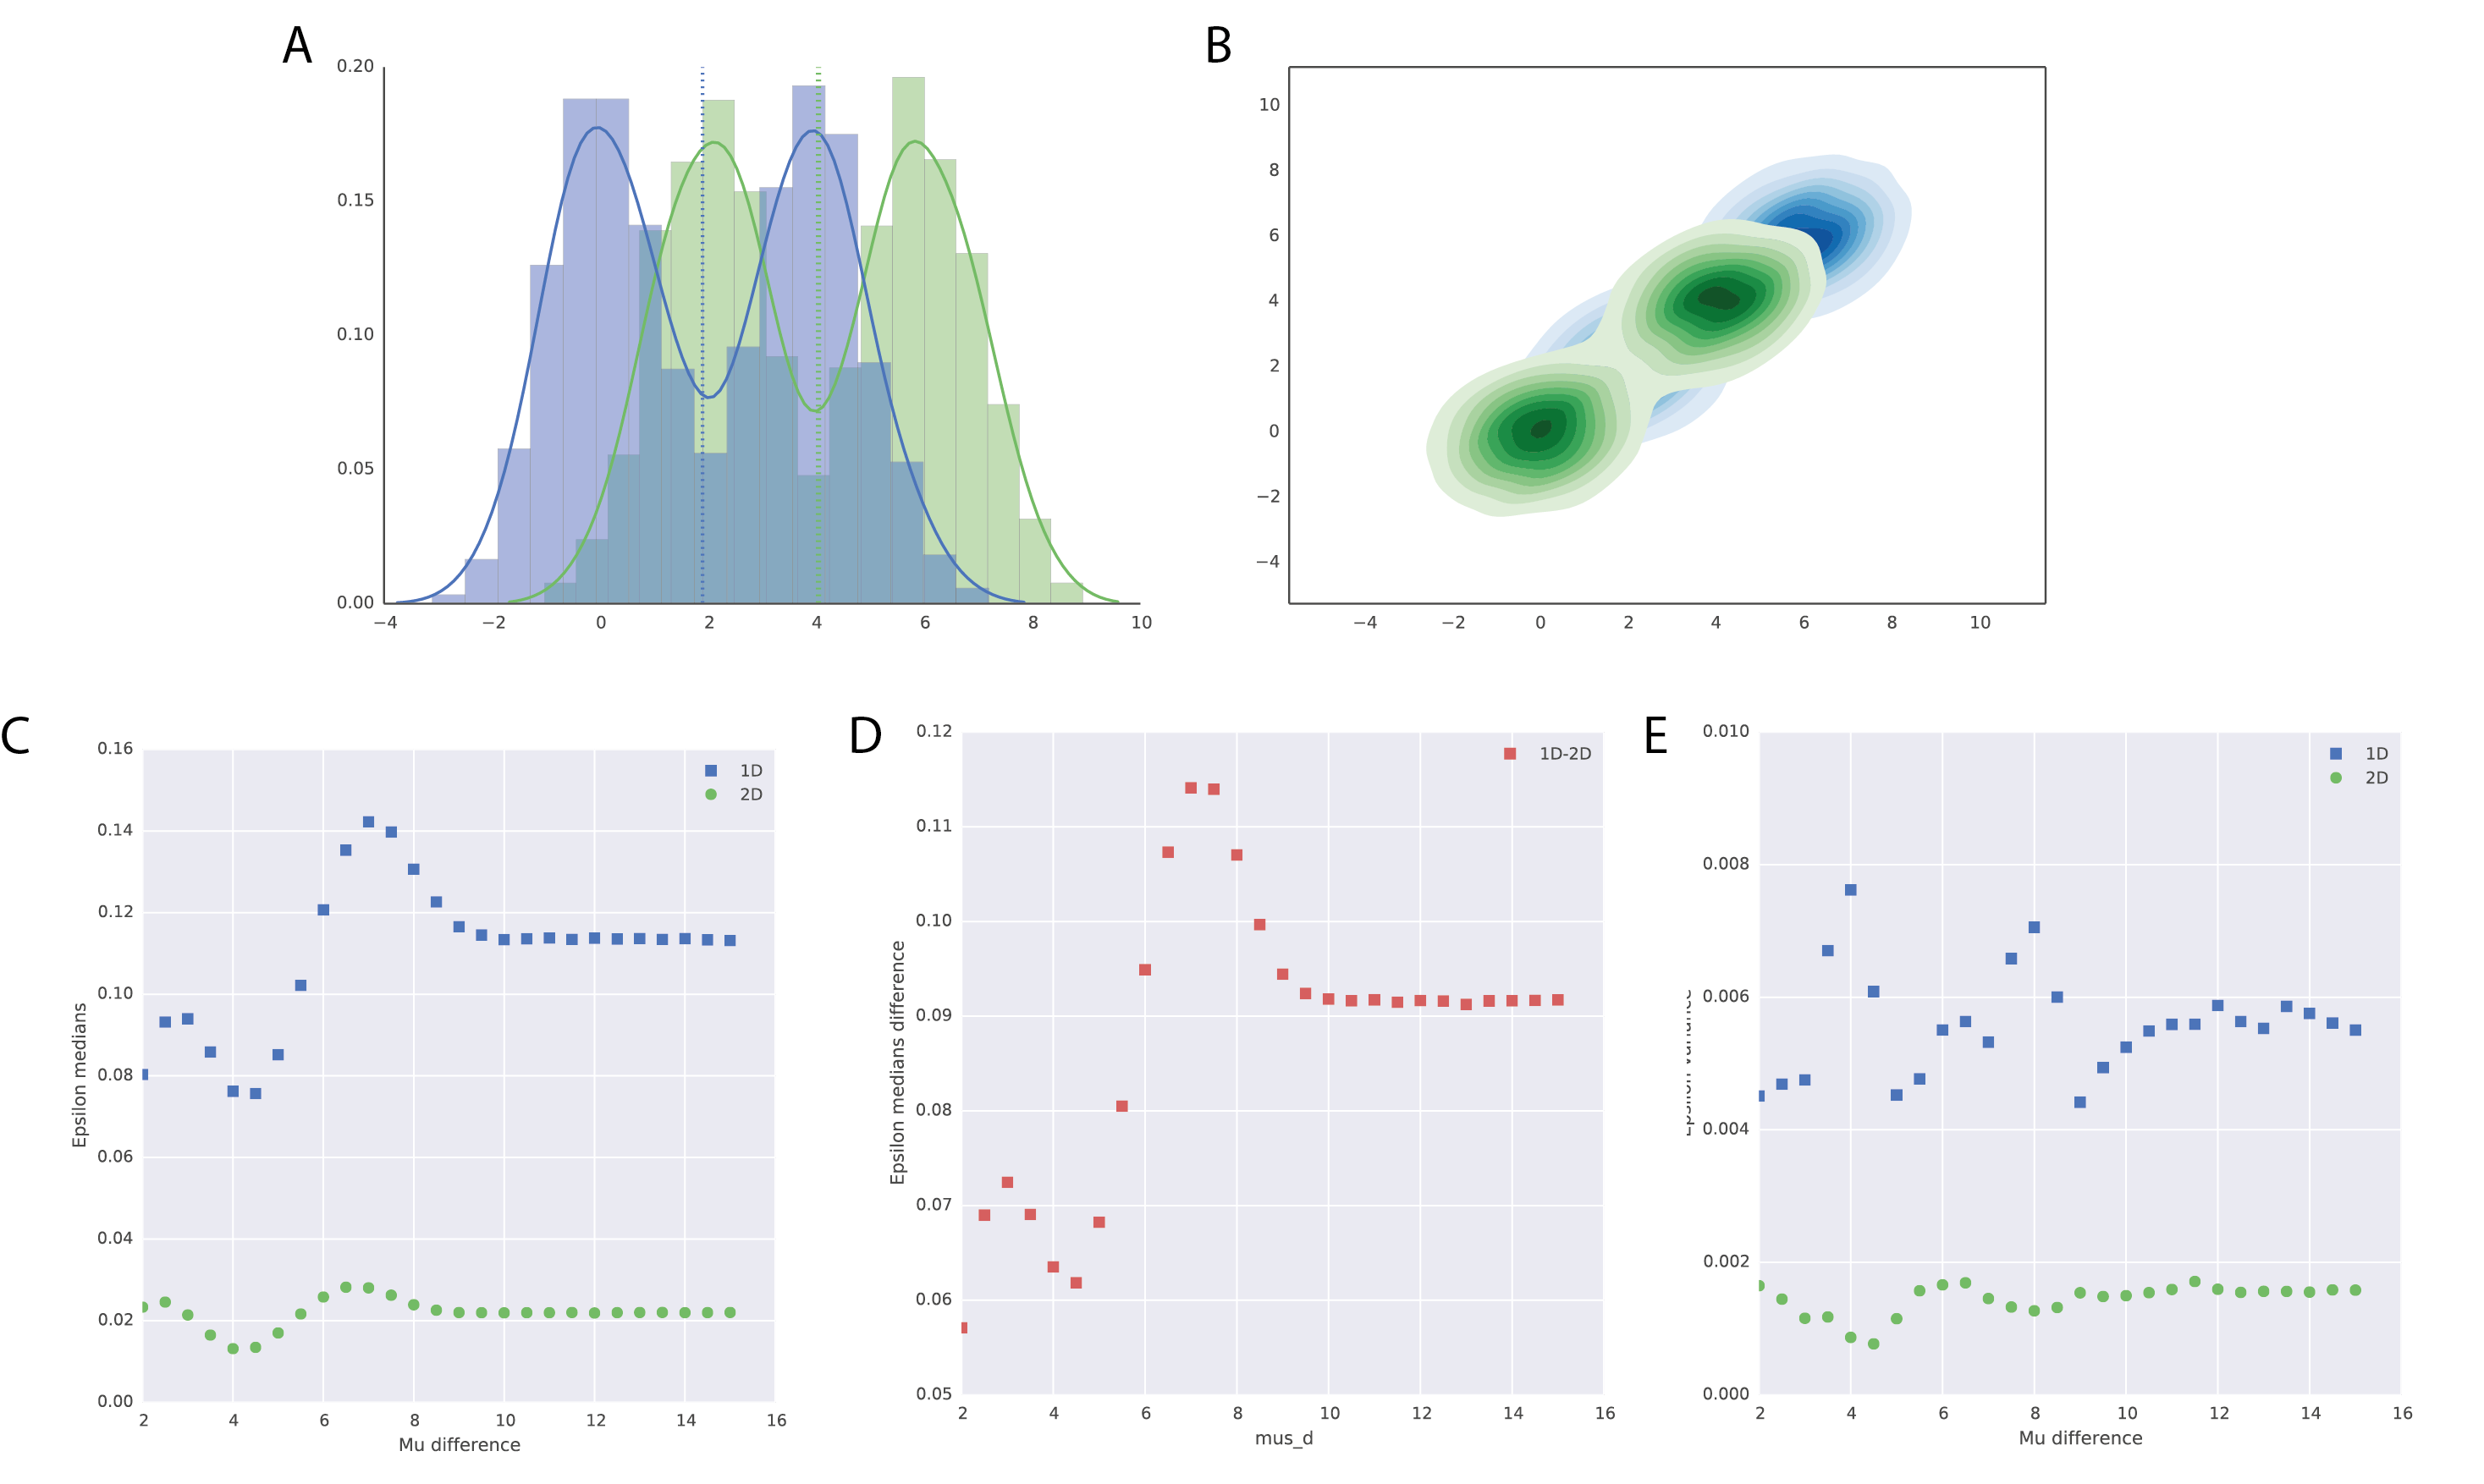
\includegraphics[scale=0.6]{chapterABCFlow/images/multimodal_musd.png}
\caption[LoF caption]{Comparing the 1D and 2D distances between bimodal distributions. (A) and (B) show samples of the bimodal distributions compared in 1D and 2D respectively with a $\mu$ difference of 4 between simulations and data. (C,D) The range by which epsilon median and variance varies as the difference between the $\mu$ of the distributions increases.}
\label{fig:multimodal_musd}
\end{figure}
\clearpage


 \subsubsection{Comparing bimodal and normal distributions}
Finally, we study how the distances perform when comparing a bimodal with a normal distribution. We test the distances by using a bimodal distribution and a series of normal distributions with increasing $\mu$, in 1D and 2D. We find that epsilon is the lowest when the $\mu$ of the normal distribution corresponds to the $\mu$ of one of the two peaks in the bimodal distribution and the highest when there is no overlap between the distributions. 


\begin{figure}[htbp]
\centering
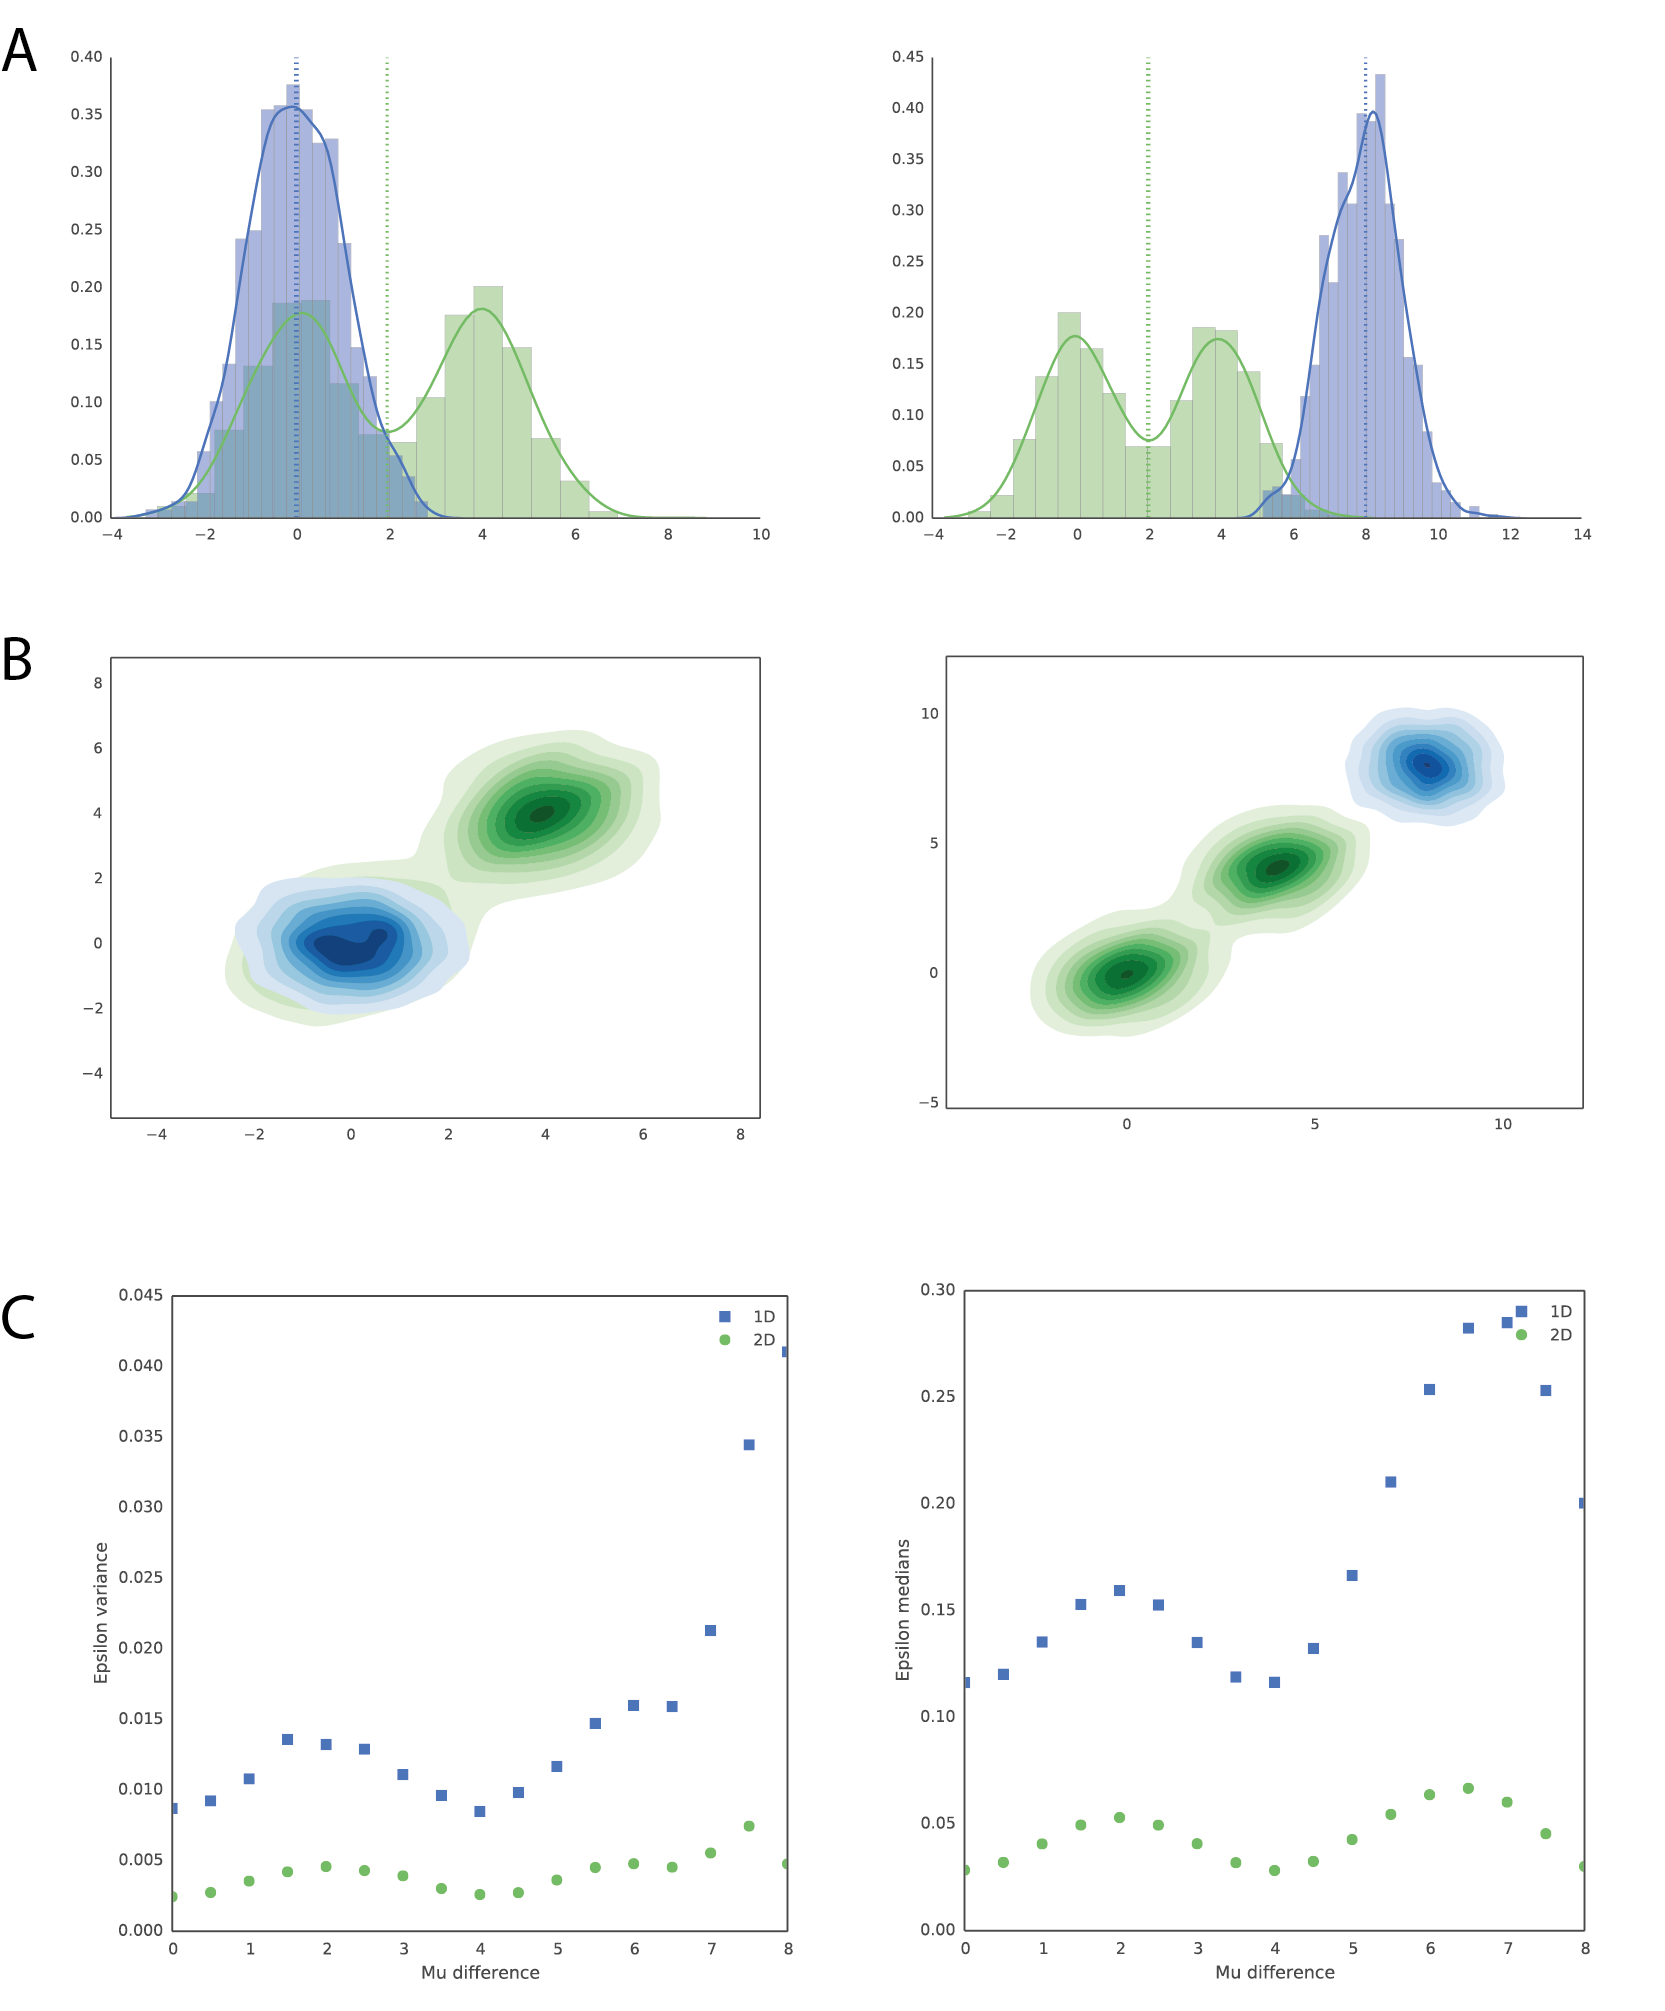
\includegraphics[scale=0.6]{chapterABCFlow/images/multimodal_v_normal.png}
\caption[LoF caption]{Comparing a multimodal to a normal distribution, in 1D and 2D. (A, B) We vary the $mu$ of the normal distribution from equal to the $\mu$ of the first peak of the bimodal distribution to beyond the range of the bimodal distribution. (C) We find that epsilon median and variance are at the lowest when the $\mu$ of the normal distribution is equal to the $\mu$ of one of the peaks of the bimodal distribution. }
\label{fig:multimodal_v_normal}
\end{figure}



\subsection{Applying ABC-Flow to simulated Gardner data}

\begin{figure}[htbp]
\centering
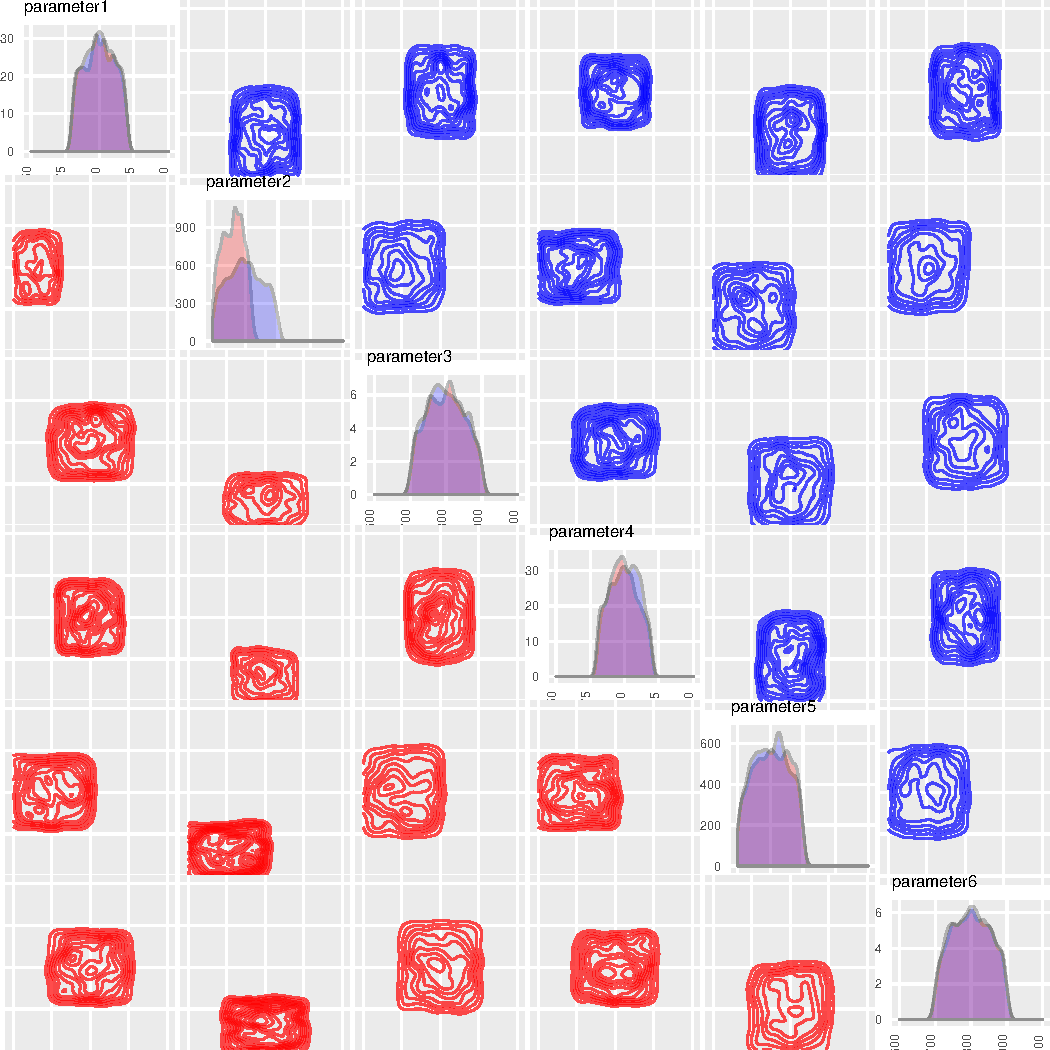
\includegraphics[scale=0.6]{chapterABCFlow/images/posterior_comparison_1D_2D.pdf}
\caption{Comparing the fit in 1D (red) Vs 2D (blue) in ABC-Flow, when $\epsilon$=0.1. }
\label{fig:1d-v-2d}
\end{figure}
\clearpage
In order to improve the identifiability of the parameters in the 2D case, we lower the final $\epsilon$:
\begin{figure}[htbp]
\centering
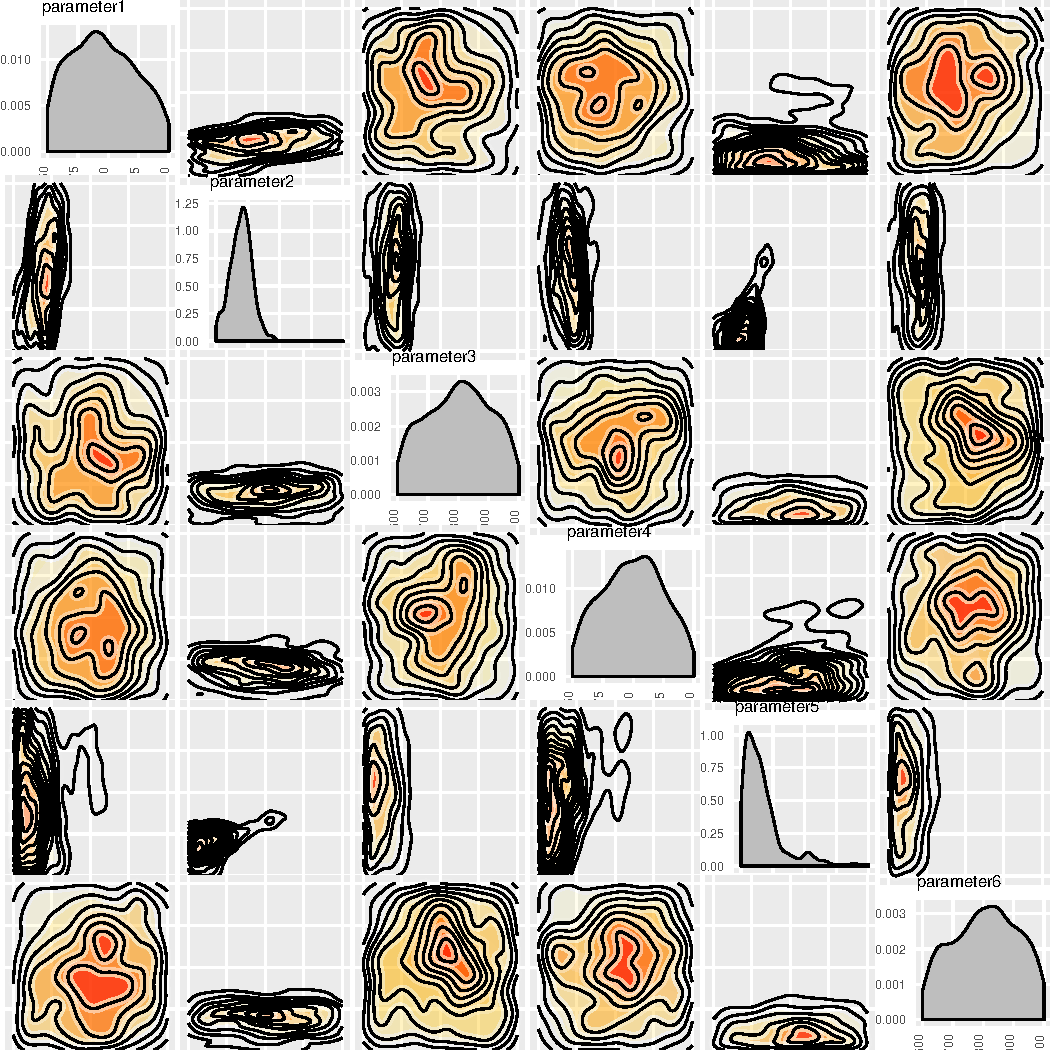
\includegraphics[scale=0.6]{chapterABCFlow/images/posterior_2d_4.pdf}
\caption[LoF caption]{$\epsilon$=0.00001.}
\label{fig:2d-e-0-00001}
\end{figure}
We find increased identifiability for parameters 2 and 5. Next we will use this epsilon in the 1D case.

\clearpage


\subsection{Applying ABC-Flow to experimental toggle switch data}
 
 
  \subsubsection{\acrshort{atc} induction}
 
 
 \begin{figure}[htbp]
\centering
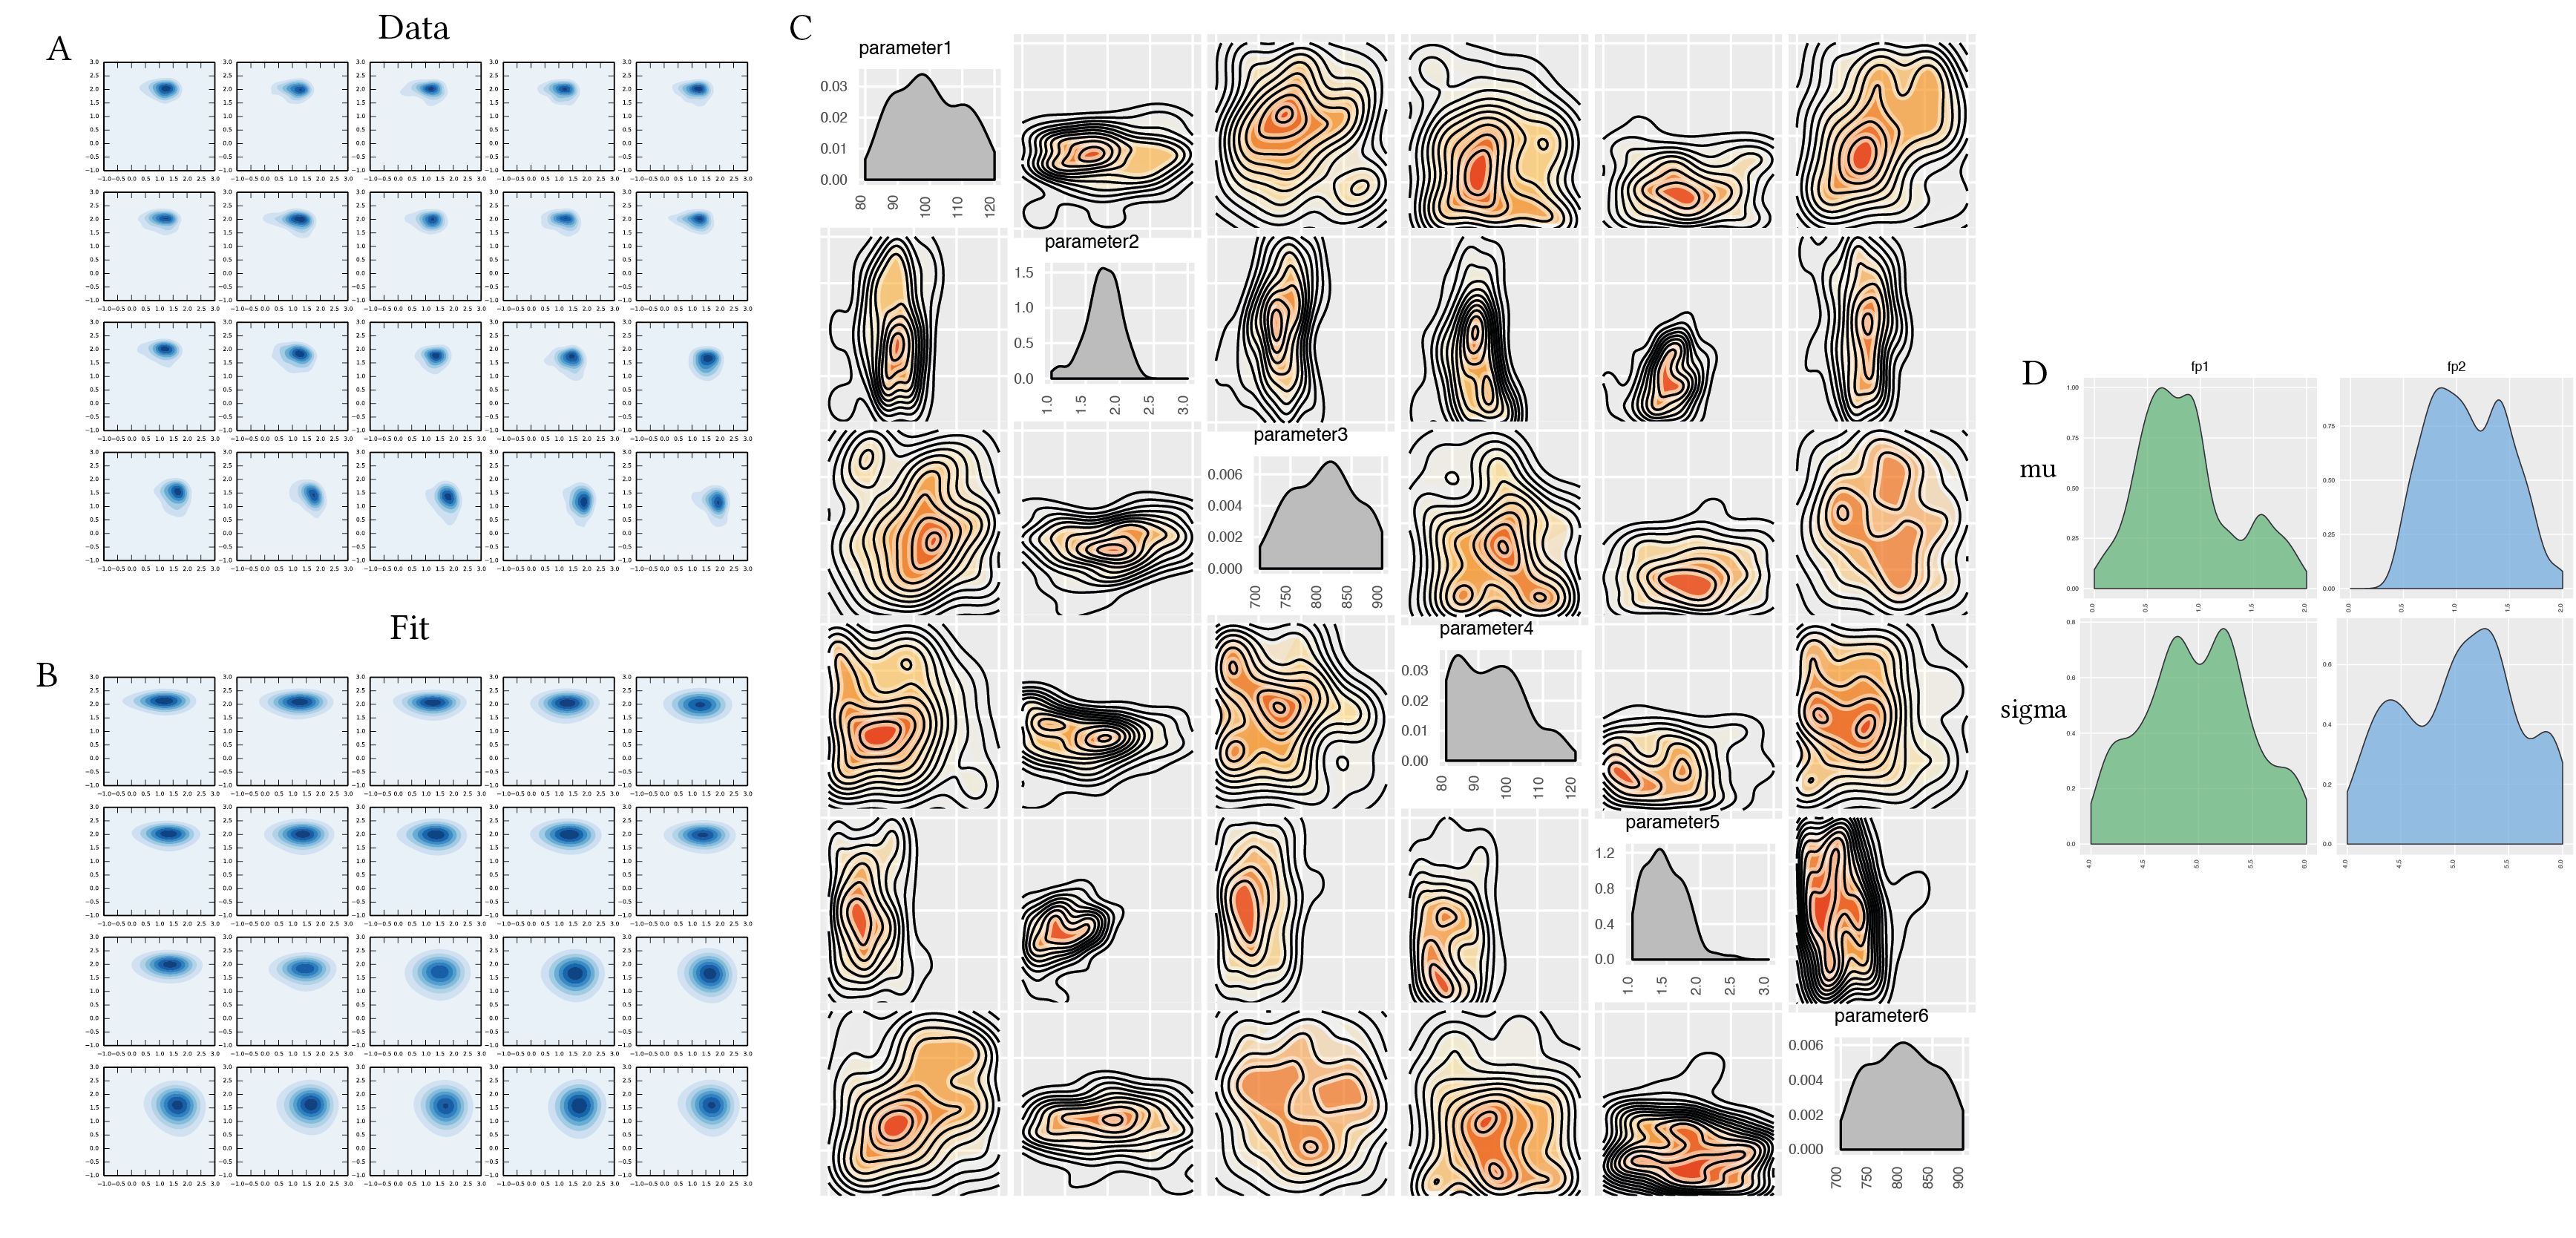
\includegraphics[scale=0.5]{chapterABCFlow/images/real_dat/real_dat_2D.png}
\caption[LoF caption]{Real data 2D fit}
\label{fig:real_dat_2d}
\end{figure}
\clearpage
\subsubsection{\acrshort{iptg} induction}
\subsection{Conclusions}

 
 